% ==============================================================================
% Contrastive Field Probing for Finite-Depth Ising Quantum Circuits:
% Non-Equilibrium Reciprocity, Shot-Budget Scaling, and 128-156-Qubit Hardware Audits
% Self-contained LaTeX manuscript (all tables inline; compiles cleanly with pdflatex).
% ==============================================================================
\pdfoutput=1
\documentclass[11pt]{article}

\usepackage[utf8]{inputenc}
\usepackage[T1]{fontenc}
\usepackage{lmodern}
\usepackage[margin=1in]{geometry}
\usepackage{microtype}
\usepackage{amsmath,amssymb,amsthm,mathtools}
\usepackage{booktabs}
\usepackage{multirow}
\usepackage{array}
\usepackage{graphicx}
\usepackage{subcaption}
\usepackage{xcolor}
\usepackage{algorithm}
\usepackage{algorithmic}
\usepackage{enumitem}
\usepackage{placeins}
\usepackage{tikz}
\usetikzlibrary{arrows.meta,positioning,calc,shapes.geometric,fit,backgrounds}

\usepackage[colorlinks=true,citecolor=blue!60!black,linkcolor=blue!60!black,urlcolor=blue!60!black,
  pdftitle={Constant-Circuit Contrastive Probing for Ising Quantum Generative Models},
  pdfauthor={Mohammad Shahid Chaudhary}]{hyperref}

% ---- Typography & Float Layout ----
\setlength{\parindent}{0pt}
\setlength{\parskip}{0.45em}
\renewcommand{\topfraction}{0.92}
\renewcommand{\bottomfraction}{0.92}
\renewcommand{\textfraction}{0.06}
\renewcommand{\floatpagefraction}{0.82}
\setlength{\textfloatsep}{10pt plus 2pt minus 2pt}
\setlength{\floatsep}{10pt plus 2pt minus 2pt}
\setlength{\intextsep}{10pt plus 2pt minus 2pt}
\makeatletter
\setlength{\@fptop}{0pt}
\setlength{\@fpsep}{12pt}
\setlength{\@fpbot}{0pt plus 1fil}
\makeatother

\definecolor{qerblue}{HTML}{0072B2}
\definecolor{qerorange}{HTML}{E69F00}
\definecolor{qerred}{HTML}{D55E00}
\definecolor{qergreen}{HTML}{009E73}
\definecolor{qerpurple}{HTML}{CC79A7}
\definecolor{slotbg}{HTML}{F7F9FC}

\newtheorem{proposition}{Proposition}
\newtheorem{remark}{Remark}

\begin{document}

% ---- Title Block ----
\begin{center}
  \rule{\linewidth}{1.6pt}\\[0.65em]
  {\Large\bfseries Constant-Circuit Contrastive Probing\\[0.25em]
  for Ising Quantum Generative Models}\\[0.65em]
  \rule{\linewidth}{0.7pt}\\[0.75em]
  {\large Mohammad Shahid Chaudhary}\\[0.15em]
  {\normalsize Independent Researcher}\\
  {\small\texttt{shahidchaudhary9@protonmail.com}}
\end{center}

\vspace{0.2em}
\begin{abstract}
When can a constant-circuit-count ($\mathcal{O}(1)$ in parameter count $P$) contrastive perturbation train finite-depth Ising quantum circuits under tight measurement shot budgets, and where does non-equilibrium reciprocity break down? We study \textbf{Quantum Equilibrium-Response Probing (\texttt{QER} / \texttt{QER-Res})}, which applies symmetric $\pm\beta$ nudges only to visible longitudinal fields of finite-depth Ising circuits ($Z_i, Z_u Z_v$ generators interleaved with fixed $R_X$ mixers) and reads simultaneous updates for all $P$ biases and two-qubit couplers from computational-basis bitstrings in $2$--$3$ circuits per sample ($175\times$--$221\times$ fewer circuits/sample than $2P$ finite-difference parameter shift at $128$--$156$ qubits). Rather than violating $\Omega(P)$ query bounds for exact quantum backpropagation, \texttt{QER} stays outside their hypotheses by restricting to commuting diagonal generators and accepting a biased forward-sensitivity surrogate whose practical advantage over constant-query SPSA lies in finite-shot signal-to-noise ratio (SNR). First, we prove analytically at depth $L{=}1$ that forward sensitivity (JVP) and true parameter gradients (VJP) diverge even as $\beta{\to}0$ via an explicit Hebbian cross-term, and we map the resulting breakdown across $6$--$14$-qubit GPU simulations: off-diagonal visible-field reciprocity remains $+0.942$--$+0.993$ at $L{=}4$, whereas $ZZ$ coupler alignment starts near $+0.998$ at small weights, undergoes a transient cubic phase inversion at intermediate weights, and settles at $+0.450$ under noisy finite-$\beta$ operation (vs.\ $-0.379$ clean $\beta{\to}0$). Second, across $3$-seed $6$--$14$-qubit benchmarks, $3$-circuit \texttt{QER-Res} maintains $+0.882{\to}+0.841$ $4\text{k}$-shot gradient SNR ($>4\times$ above $100$-direction SPSA and coordinate PSR), reaches $85.2\pm 0.5\%$ satisfied bonds on $12$-qubit Heavy-Hex spin glasses (within $1.5\text{ pp}$ of noiseless \texttt{Exact-AD} at $86.7\pm 3.1\%$), and stays flat at $85.3\%{\to}84.3\%$ up to $1.5\%$ two-qubit CNOT depolarizing error while all-to-all layouts collapse to $8.9\%$. Third, scaling to live $128$--$156$-qubit IBM Heron R2 (\texttt{ibm\_kingston}, $0$ SWAPs) hardware ($31\text{k}$--$39\text{k}$ training shots), raw \texttt{QER-Res} reaches $83.0\%$ and $87.7\%$ satisfied bonds across two $128$-qubit $\pm J$ spin-glass instances ($78.0\%$ on the full $156$-qubit chip; $r{=}+0.905$--$+0.945$ edge-correlation fidelity vs.\ held-out Simulated Annealing) and $75.1\%$ vs.\ $47.5\%$ promoter activity over live SPSA on $128$-qubit DNA. Finally, we pair every benchmark with diagnostic negative controls—exposing session-specific hardware-drift sector locking ($\overline{|m_i|}{=}0.485$ even at $\boldsymbol{\theta}{=}\mathbf{0}$), classical sign-Hebbian equivalence on standalone spin glasses, $1$-body dominance on $L{=}2$ DNA, linear conditioning shortcuts on whitened vision latents, and Straight-Through Estimator (\texttt{STE}) parity when quantum weights are frozen.
\end{abstract}

% ==============================================================================
\section{Introduction}
\label{sec:intro}
% ==============================================================================
Optimizing parameterized quantum circuits on Noisy Intermediate-Scale Quantum (NISQ) processors is governed by a sharp trade-off between circuit query complexity and finite-shot estimator variance. Analytic Parameter-Shift Rules (PSR)~\cite{mitarai2018psr,schuld2019psr} require $2LP$ shifted circuit evaluations per sample across $L$ layers and $P$ parameters, and information-theoretic quantum backpropagation bounds~\cite{abbas2023qbp} prove that achieving classical $\mathcal{O}(1)$ query scaling for \emph{unbiased exact gradients} on general circuits is impossible without coherent multi-copy access. On a $128$-qubit Heavy-Hex Ising circuit ($P{=}263$), even layer-tied finite-difference PSR ($2P{=}526$ circuits/sample) cannot complete a single update within a $38{,}016$-shot budget. Doubly stochastic randomized-coordinate PSR~\cite{sweke2020sgd} and adaptive shot-allocation schemes (\texttt{iCANS}~\cite{kubler2020icans}, \texttt{Rosalin}~\cite{arrasmith2020rosalin}) reduce per-step cost by probing random coordinate subsets with $1$--$4$ shots, yet still require $\Omega(P)$ queries per full sweep and suffer severe finite-shot noise when single-parameter loss shifts scale as $\mathcal{O}(1/n)$. Conversely, Simultaneous Perturbation Stochastic Approximation (SPSA)~\cite{spall1992spsa,kandala2017vqe} and directional forward-gradient estimators~\cite{coyle2026forward} use $\mathcal{O}(1)$ circuits per step, but projecting a scalar loss difference onto $P$ simultaneous random directions incurs $\mathcal{O}(P/c_k^2)$ mask-crosstalk variance.

In classical energy-based learning, Equilibrium Propagation (EP)~\cite{scellier2017ep,laydevant2024ep,scellier2024ep} avoids coordinate-wise perturbations by nudging visible outputs toward targets and reading simultaneous weight updates from local contrastive differences at thermal or fixed-point equilibrium. Recent quantum generalizations extend EP to stationary or ground-state quantum systems by invoking exact Onsager reciprocity~\cite{wanjura2025qep} or ground-state energy functionals~\cite{scellier2026qep}. However, gate-based NISQ processors typically execute \emph{non-stationary, finite-depth Trotter circuits}~\cite{farhi2014qaoa} rather than relaxing to thermal or ground-state equilibrium. In finite-depth unitary dynamics, it is unclear a priori whether nudging visible longitudinal fields provides a valid gradient surrogate for internal two-qubit couplers, when reciprocity holds or fails, and whether the resulting $\mathcal{O}(1)$-circuit updates remain useful on $>100$-qubit superconducting hardware.

\paragraph{Scope and Chronological Roadmap.}
We address this question systematically through \textbf{Quantum Equilibrium-Response Probing (\texttt{QER} / \texttt{QER-Res})}, organizing the paper in four chronological stages from exact analytical theory to $156$-qubit hardware audits:
\begin{enumerate}[leftmargin=1.4em,itemsep=2pt,topsep=2pt]
  \item \textbf{Method \& Non-Equilibrium Reciprocity Theory (\S\ref{sec:method}):} For finite-depth Ising circuits whose trainable weights multiply commuting diagonal operators ($Z_i, Z_u Z_v$) interleaved with fixed $R_X$ mixers, symmetric $\pm\beta$ visible-field nudges cancel even-order curvature to $\mathcal{O}(\beta^2)$ and yield simultaneous updates for all $P$ biases and couplers from computational-basis bitstrings in $2$ circuits/sample ($3$ circuits under residual MSE nudging, \texttt{QER-Res}), paired with $\beta_2$-normalized \texttt{StabilizedAdam} stepping and inverse-OLS readout calibration. Proposition~\ref{prop:centered_bias} proves analytically at $L{=}1$ why forward sensitivity (JVP) and transpose sensitivity (VJP) diverge even as $\beta{\to}0$ via an explicit Hebbian cross-term, while identifying the qualitative small-$|\boldsymbol{\theta}|$ Kubo alignment regime and its continuous-time / non-stationary caveats.
  \item \textbf{Controlled $6$--$14$-Qubit Reciprocity, SNR, \& $2$Q-Noise Verification (\S\ref{sec:sim_controls}):} Before scaling to hardware where exact gradients are intractable, we audit \texttt{QER-Res} on $6$--$14$-qubit GPU simulations against noiseless same-circuit \texttt{Exact-AD}. We show that strictly off-diagonal visible-field reciprocity holds at $+0.942$--$+0.993$ ($L{=}4$), whereas $ZZ$ coupler reciprocity starts near $+0.998$, undergoes a transient cubic phase inversion at intermediate weights ($\max|\theta|{\approx}0.89$), and settles at $+0.450$ under NISQ $\beta{=}0.45$ (vs.\ $-0.379$ clean $\beta{\to}0$). Across $n{=}6{\to}14$ ($P{=}21{\to}105$), \texttt{QER-Res} maintains $+0.882{\to}+0.841$ $4\text{k}$-shot gradient SNR ($>4\times$ above $100$-direction SPSA and Coord-PSR), reaches $85.2\pm 0.5\%$ satisfied bonds on $12$q Heavy-Hex spin glasses (vs.\ $86.7\pm 3.1\%$ noiseless \texttt{Exact-AD}), stays flat at $85.3\%{\to}84.3\%$ up to $p_{2\text{q}}{=}1.5\%$ CNOT error (where all-to-all collapses to $8.9\%$), and learns multi-qubit $ZZ$ structure on zero-shortcut $12$--$14$q benchmarks.
  \item \textbf{Live $128$--$156$-Qubit IBM Heron R2 Hardware Audits (\S\ref{sec:heron}):} Scaling past the $\sim 26$-qubit statevector simulation wall on \texttt{ibm\_kingston} ($0$ SWAPs), raw live \texttt{QER-Res} reaches $83.0\%$ (\texttt{seed=42}) and $87.7\%$ (\texttt{seed=43}) satisfied bonds on $128$-qubit frustrated $\pm J$ spin glasses ($78.0\%$ on the full $156$-qubit chip; $r{=}+0.905$--$+0.945$ two-point correlation fidelity vs.\ held-out Simulated Annealing), outperforming equal-shot live \texttt{Coord-PSR} ($46.1\%$), untrained QPU ($51.9\%$), \texttt{no-zz} ($61.1\%$), and $96$-direction \texttt{SPSA} ($62.9\%$ / $49.1\%$), as well as beating live Chain-Rule \texttt{SPSA} by $+27.6\text{ pp}$ promoter activity on $128$-qubit ($64\text{ bp}$) Human Promoter DNA ($75.1\%$ vs.\ $47.5\%$).
  \item \textbf{Forensic Bitstring Diagnostics \& Negative Controls (\S\ref{sec:heron_audit} \& \S\ref{sec:discussion}):} Rather than overclaiming quantum generative advantage, we audit raw hardware bitstrings and saved weights to expose five concrete boundaries: (i) standard deterministic iterative sampling on \texttt{ibm\_kingston} locks into a single $\mathbb{Z}_2$ sector ($\overline{|m_i|}{=}0.485$ even at $\boldsymbol{\theta}{=}\mathbf{0}$) due to session-specific in-circuit hardware drift ($r{=}+0.318$ same-day vs.\ $+0.052$ cross-day), which live batch-centered $\mathbb{Z}_2$ debiasing mitigates ($\overline{|m_i|}{=}0.093, r{=}+0.956, 77.8\%$ satisfied bonds at $32$ eval shots/step); (ii) on standalone sparse spin glasses, learned couplers closely track a uniform signed Hebbian template ($r{=}+0.995$) while classical inverse-Ising Gibbs solvers reach $90.3\%$--$94.1\%$; (iii) live $128$q DNA \texttt{no-zz} ($81.9\%$ activity) proves $1$-body positional fields dominate $L{=}2$ DNA; (iv) whitened vision autoencoders admit trivial linear conditioning shortcuts (\texttt{wcond-only} $100.0\%$ MNIST); and (v) a $0$-backward-shot Straight-Through Estimator (\texttt{STE}) trails hybrid \texttt{QERLayer} by only $\sim 0.5\sigma$ when quantum weights are frozen.
\end{enumerate}

% ==============================================================================
\section{Method and Non-Equilibrium Reciprocity Theory}
\label{sec:method}
% ==============================================================================

\subsection{Parameterized Ising-Mixer Circuit and Iterative Denoising Testbed}
\label{sec:denoiser}
Consider a discrete spin configuration or bounded vector $\mathbf{x}_0 \in [-1,1]^D$. As a standardized multi-step testbed for training and evaluating parameterized quantum circuits, we corrupt $\mathbf{x}_0$ over $T{=}4$ discrete cosine noise steps ($\bar{\alpha}_t \in [0.02, 0.98]$)~\cite{sohldickstein2015,ho2020ddpm} via $\mathbf{x}_t = \operatorname{clip}_{[-1,1]}(\sqrt{\bar{\alpha}_t}\mathbf{x}_0 + \sqrt{1-\bar{\alpha}_t}\boldsymbol{\epsilon})$ with $\boldsymbol{\epsilon}\sim\mathcal{N}(\mathbf{0}, \sigma_{\text{diff}}^2\mathbf{I})$ ($\sigma_{\text{diff}}{=}0.70$). The quantum circuit takes $(\mathbf{x}_t, \tau{=}t/T)$ (plus optional class conditioning $\mathbf{c}\in\mathbb{R}^K$) and outputs bounded computational-basis expectations $\langle Z_i \rangle \in [-1,1]$ to predict $\hat{\mathbf{x}}_0 \approx \mathbf{x}_0$. Iterative inference steps from $t{=}T$ down to $1$ via $\mathbf{x}_{t-1} = \operatorname{clip}_{[-1,1]}(\sqrt{\bar{\alpha}_{t-1}}\hat{\mathbf{x}}_0 + \sqrt{1-\bar{\alpha}_{t-1}}\sigma_{\text{step}}\boldsymbol{\xi}_t)$, returning $\hat{\mathbf{x}}_0$ (or $\operatorname{sign}(\hat{\mathbf{x}}_0)$ for discrete spins) at $t{=}1$. We use this $4$-step denoising loop purely as an operational circuit-training testbed (we also evaluate single-shot unconditioned circuits directly in \S\ref{sec:heron_audit} and standalone non-diffusion classification layers in \S\ref{sec:hybrid_sim}).

Starting from the uniform superposition $\rho_0 = |\psi_0\rangle\langle\psi_0|$ with $|\psi_0\rangle = H^{\otimes n}|0\rangle^{\otimes n}$ over $n = n_{\text{vis}}+n_{\text{hid}}$ qubits and coupling graph $G=(V,E)$, each layer $\ell \in \{1,\dots,L\}$ applies the noisy channel
\begin{equation}
  \mathcal{M}_\ell(\rho) = \mathcal{E}_{\text{depol}}^{(p_{\text{depol}})}\!\left(V_\ell\,\rho\,V_\ell^\dagger\right), \qquad V_\ell = U_X^{(\ell)}(\tau)\,U_Z^{(\ell)}(\mathbf{h},\mathbf{J}),
  \label{eq:mold_shake}
\end{equation}
alternating a parameterized diagonal Ising rotation (\emph{Mold}) with a fixed transverse mixer pulse (\emph{Shake}):
\begin{equation}
  U_Z^{(\ell)}(\mathbf{h},\mathbf{J}) = \exp\!\left[-i\,\frac{g_\ell^{\text{mold}}}{2}\!\left(\sum_{i=1}^n h_i Z_i + \sum_{(u,v)\in E} J_{uv} Z_u Z_v\right)\right], \qquad
  U_X^{(\ell)}(\tau) = \bigotimes_{i=1}^n R_X^{(i)}\!\left(\theta_\ell^{\text{shake}}(\tau)\right).
  \label{eq:uz_ux}
\end{equation}
Here the longitudinal gain ramps linearly with layer depth as $g_\ell^{\text{mold}} = 2\Delta t\,\beta_{\text{temp}}(\ell/L)$ (with $\Delta t{=}0.42$ and $\beta_{\text{temp}}{=}1.25$), while the fixed transverse mixer angle decays along depth: $\theta_\ell^{\text{shake}}(\tau) = s_{\text{shake}}\cdot 2\Delta t(1 - f_{\text{fin}}\ell/L)(0.6 + 0.4\tau)$ ($s_{\text{shake}}{=}2.2$, $f_{\text{fin}}{=}0.70$). Input states $\mathbf{x}_t$ enter the visible longitudinal fields via $\lambda(\tau) = 0.28 + 0.52(1-\tau)$. When hidden ancilla qubits are present ($n_{\text{hid}}>0$), initializing all parameters at zero traps $\langle Z_h\rangle \equiv 0$ by $\mathbb{Z}_2$ spin-flip symmetry; initializing $J_{vh}\sim\mathcal{N}(0,0.08^2)$ and $b_h\sim\mathcal{N}(0,0.04^2)$ breaks this symmetry at step~$1$.

\begin{figure}[t!]
\centering
\resizebox{\textwidth}{!}{%
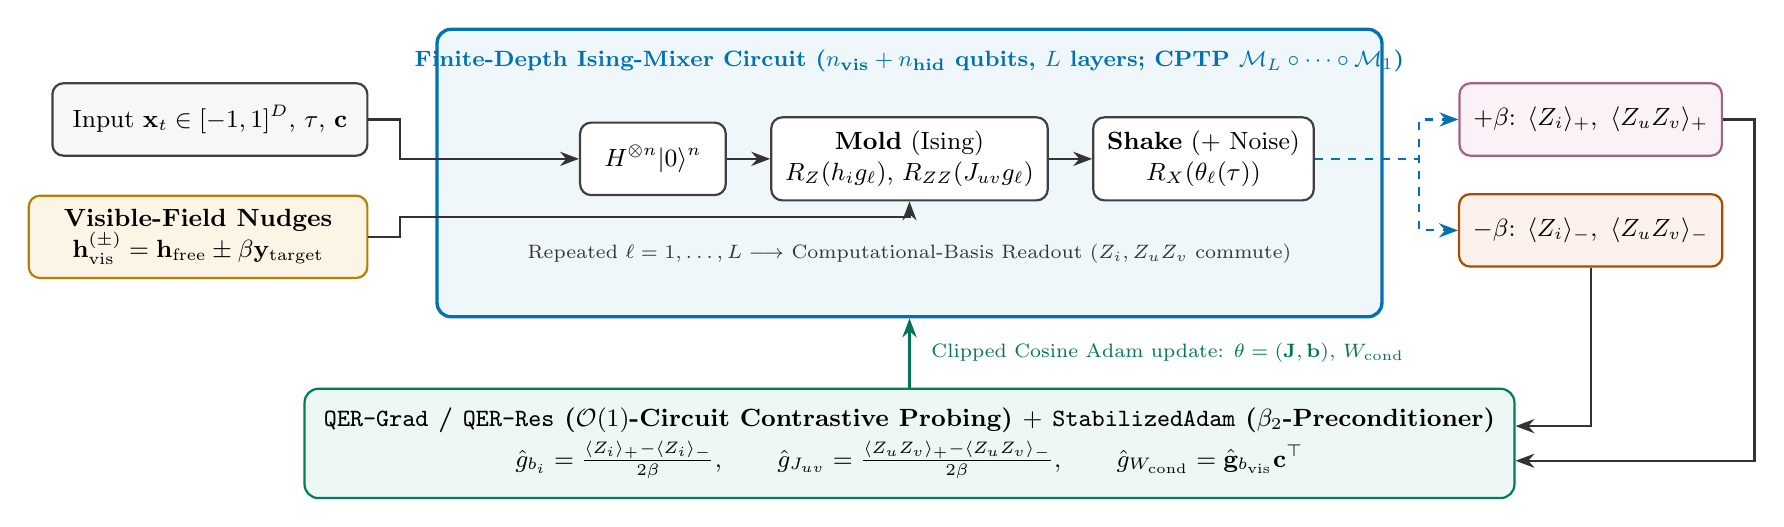
\begin{tikzpicture}[
    font=\small,
    box/.style={draw=black!75, rounded corners=4pt, fill=white, align=center, minimum height=0.92cm, inner sep=5pt, thick},
    qpu/.style={draw=qerblue, rounded corners=5pt, fill=qerblue!6, align=center, inner sep=7pt, very thick},
    opt/.style={draw=qergreen!80!black, rounded corners=5pt, fill=qergreen!7, align=center, inner sep=7pt, thick},
    arr/.style={-{Stealth[length=2.4mm]}, thick, color=black!80},
    darr/.style={-{Stealth[length=2.4mm]}, thick, dashed, color=qerblue}
]
\node[qpu, minimum width=12.0cm, minimum height=3.65cm] (qpu_box) at (0,0) {};
\node[anchor=north, yshift=-0.16cm, font=\footnotesize\bfseries\color{qerblue}] at (qpu_box.north) {Finite-Depth Ising-Mixer Circuit ($n_{\text{vis}}+n_{\text{hid}}$ qubits, $L$ layers; CPTP $\mathcal{M}_L\circ\cdots\circ\mathcal{M}_1$)};
\node[box, fill=white, minimum width=2.65cm] (mold) at (0.0, 0.18) {\textbf{Mold} (Ising)\\$R_Z(h_i g_\ell)$, $R_{ZZ}(J_{uv} g_\ell)$};
\node[box, fill=white, left=0.55cm of mold, minimum width=1.85cm] (init) {$H^{\otimes n}|0\rangle^n$};
\node[box, fill=white, right=0.55cm of mold, minimum width=2.35cm] (shake) {\textbf{Shake} (+ Noise)\\$R_X(\theta_\ell(\tau))$};
\node[below=0.42cm of mold, font=\scriptsize\color{black!80}] {Repeated $\ell=1,\dots,L \longrightarrow$ Computational-Basis Readout ($Z_i, Z_u Z_v$ commute)};
\node[box, fill=gray!6, anchor=east, minimum width=4.0cm] (inp) at ($(qpu_box.west)+(-0.85, 0.68)$) {Input $\mathbf{x}_t \in [-1,1]^D$, $\tau$, $\mathbf{c}$};
\node[box, below=0.48cm of inp.south east, anchor=north east, fill=qerorange!10, draw=qerorange!80!black, minimum width=4.3cm] (nudge) {\textbf{Visible-Field Nudges}\\$\mathbf{h}_{\text{vis}}^{(\pm)} = \mathbf{h}_{\text{free}} \pm \beta \mathbf{y}_{\text{target}}$};
\node[box, anchor=west, fill=qerpurple!10, draw=qerpurple!80!black, minimum width=3.2cm] (obs_p) at ($(qpu_box.east)+(0.95, 0.68)$) {$+\beta$: $\langle Z_i\rangle_+,\ \langle Z_u Z_v\rangle_+$};
\node[box, below=0.46cm of obs_p, fill=qerred!8, draw=qerred!80!black, minimum width=3.2cm] (obs_m) {$-\beta$: $\langle Z_i\rangle_-,\ \langle Z_u Z_v\rangle_-$};
\node[opt, below=0.88cm of qpu_box, minimum width=12.0cm] (qeropt) {%
  \textbf{\texttt{QER-Grad} / \texttt{QER-Res} ($\mathcal{O}(1)$-Circuit Contrastive Probing) $+$ \texttt{StabilizedAdam} ($\beta_2$-Preconditioner)}\\[0.2em]
  $\hat{g}_{b_i} = \frac{\langle Z_i\rangle_+ - \langle Z_i\rangle_-}{2\beta},\qquad \hat{g}_{J_{uv}} = \frac{\langle Z_u Z_v\rangle_+ - \langle Z_u Z_v\rangle_-}{2\beta},\qquad \hat{g}_{W_{\text{cond}}} = \hat{\mathbf{g}}_{b_{\text{vis}}}\mathbf{c}^\top$
};
\draw[arr] (inp.east) -- ++(0.40,0) |- (init.west);
\draw[arr] (nudge.east) -- ++(0.40,0) |- ([yshift=-0.20cm]mold.south) -- (mold.south);
\draw[arr] (init) -- (mold); \draw[arr] (mold) -- (shake);
\coordinate (branch) at ($ (qpu_box.east)+(0.45,0) $);
\draw[darr] (shake.east) -- (branch |- shake.east) |- (obs_p.west);
\draw[darr] (shake.east) -- (branch |- shake.east) |- (obs_m.west);
\draw[arr] (obs_m.south) |- ([yshift=0.22cm]qeropt.east);
\draw[arr] (obs_p.east) -- ++(0.40,0) |- ([yshift=-0.22cm]qeropt.east);
\draw[arr, color=qergreen!75!black, very thick] (qeropt.north) -- node[right=4pt, font=\scriptsize] {Clipped Cosine Adam update: $\theta=(\mathbf{J},\mathbf{b}),\, W_{\text{cond}}$} (qpu_box.south);
\end{tikzpicture}%
}
\caption{\textbf{Contrastive Field Probing (\texttt{QER-Grad} / \texttt{QER-Res}) Architecture.} Because all trainable generators $\{Z_i, Z_u Z_v\}$ commute in the computational basis, two symmetrically nudged visible-field configurations ($\pm\beta\mathbf{y}_{\text{target}}$) yield dense simultaneous updates for all $J_{uv}$, $b_i$, and $W_{\text{cond}}$ in $\mathcal{O}(1)$ circuits independent of $P$.}
\label{fig:arch}
\end{figure}

\subsection{Constant-Circuit Contrastive Field Probing and Preconditioned Stepping}
\label{sec:qer_opt}
Collect all trainable quantum couplers and biases into $\boldsymbol{\theta}=(\mathbf{J},\mathbf{b})\in\mathbb{R}^{|E|+n}$, paired with their commuting diagonal observables $\mathcal{O}_k \in \{Z_u Z_v, Z_i\}$, alongside optional classical conditioning weights $W_{\text{cond}} \in \mathbb{R}^{n_{\text{vis}}\times K}$. Given a visible-qubit nudge direction $\mathbf{y}_{\text{target}}\in\mathbb{R}^{n_{\text{vis}}}$, contrastive field probing evaluates two visible-field configurations per sample:
\begin{equation}
  \mathbf{h}_{\text{vis}}^{(\pm)}(\mathbf{x}_t,\tau,\mathbf{c}) = \mathbf{b}_{\text{vis}} + \lambda(\tau)\mathbf{x}_t + W_{\text{cond}}\mathbf{c} \pm \beta\,\mathbf{y}_{\text{target}},
  \label{eq:contrastive_fields}
\end{equation}
while $\mathbf{J}$ and any hidden biases $\mathbf{b}_{\text{hid}}$ remain unperturbed (Figure~\ref{fig:arch}). Measuring computational-basis bitstrings over a minibatch of $M$ samples ($K_s$ shots per sign) yields empirical expectations $\hat{\boldsymbol{\mu}}^{(\pm)}$ for all $P$ diagonal operators $\{Z_u Z_v, Z_i\}$ and visible magnetizations $\hat{\mathbf{z}}_{\text{vis}}^{(\pm)}$ simultaneously:
\begin{equation}
  \hat{\mathbf{g}}_\theta = \frac{1}{M}\sum_{m=1}^M \frac{\hat{\boldsymbol{\mu}}_m^{(+)}-\hat{\boldsymbol{\mu}}_m^{(-)}}{2\beta}, \qquad
  \hat{\mathbf{g}}_{W_{\text{cond}}} = \frac{1}{M}\sum_{m=1}^M \left(\frac{\hat{\mathbf{z}}_{\text{vis},m}^{(+)}-\hat{\mathbf{z}}_{\text{vis},m}^{(-)}}{2\beta}\right)\mathbf{c}_m^\top.
  \label{eq:qer_grads}
\end{equation}
We compare two nudge modes (Algorithm~\ref{alg:qer_step}):
\begin{itemize}[leftmargin=1.4em,itemsep=1pt,topsep=1pt]
  \item \textbf{Target Nudging (\texttt{QER-Grad}, $2$ circuits/sample):} Setting $\mathbf{y}_{\text{target}}{=}\mathbf{x}_0$ probes the local response ascending the correlation objective $\mathbb{E}[\mathbf{x}_0^\top\mathbf{z}_{\text{vis}}]$, omitting the $-\frac{1}{2}\nabla_\theta\|\mathbf{z}_{\text{vis}}\|^2$ self-overlap penalty of the MSE loss $\frac{1}{2}\|\mathbf{z}_{\text{vis}}-\mathbf{x}_0\|^2$.
  \item \textbf{Residual Nudging (\texttt{QER-Res}, $3$ circuits/sample):} Measuring a free-phase expectation $\hat{\mathbf{z}}_{\text{free}}$ (at $\beta{=}0$) to form the calibrated residual $\mathbf{y}_{\text{target}} = (\mathbf{x}_0 - \hat{\mathbf{x}}_0)/g_t$ supplies the missing $-\nabla_{\mathbf{z}_{\text{vis}}}\mathcal{L}_{\text{MSE}}$ factor, acting as a $3$-circuit residual-nudged MSE surrogate.
\end{itemize}

\paragraph{Second-Moment Preconditioning (\texttt{StabilizedAdam}).}
Contrastive response magnitudes differ across $W_{\text{cond}}$, single-qubit biases $b_i$, and two-qubit couplers $J_{uv}$. Dividing by the running second moment $\sqrt{\hat{\mathbf{v}}_t}$ ($\beta_2{=}0.98$) normalizes coordinate step sizes automatically: in controlled factor-isolation tests (\S\ref{sec:discussion}), \texttt{RMSprop-Only} ($\beta_1{=}0, \beta_2{=}0.98$) matches full Adam ($96.6\%$--$99.6\%$ at $\mathrm{lr}\in[0.06,0.12]$), whereas \texttt{Momentum-Only} ($\beta_2{=}0$) drops to $37.8\%$--$87.1\%$ unless manually retuned $4\times$ higher. We pair Adam~\cite{kingma2015adam} ($\beta_1{=}0.75, \beta_2{=}0.98$) with cosine LR annealing ($\alpha_{\max}{\to}\alpha_{\min}$, which reduces seed variance by $20\times$ over constant LR), LR-coupled weight decay $(1-\eta_w\alpha_p/\alpha_{\max})$, and box clipping $[-B_c, B_c]$ to prevent $2\pi$ gate-phase wraparound.

\begin{algorithm}[t!]
\caption{\texttt{QER-Grad} ($2$-Circuit) / \texttt{QER-Res} ($3$-Circuit) Contrastive Probing + \texttt{StabilizedAdam}}
\label{alg:qer_step}
\begin{algorithmic}[1]
\small
\REQUIRE Parameters $\mathcal{P}=\{\boldsymbol{\theta}, W_{\text{cond}}\}$, minibatch $(\mathbf{x}_t, \tau, \mathbf{c}, \mathbf{x}_0)$, progress $p\in[0,1]$, radius $\beta$, bounds $[-B_c, B_c]$.
\STATE Set $\mathbf{y}_{\text{target}} \leftarrow \mathbf{x}_0$ ($2$-ckt \texttt{QER-Grad}) or measure $\hat{\mathbf{z}}_{\text{free}}$ and set $\mathbf{y}_{\text{target}} \leftarrow (\mathbf{x}_0 - \hat{\mathbf{x}}_0)/g_t$ ($3$-ckt \texttt{QER-Res}).
\STATE Evaluate QPU expectations at $+\beta$ and $-\beta$ visible-field nudges (Eq.~\eqref{eq:contrastive_fields}): $(\hat{\boldsymbol{\mu}}_m^{(\pm)}, \hat{\mathbf{z}}_m^{(\pm)})$.
\STATE Compute simultaneous surrogate updates $\hat{\mathbf{g}}_\theta, \hat{\mathbf{g}}_{W_{\text{cond}}}$ via Eq.~\eqref{eq:qer_grads}.
\STATE Set $\alpha_p \leftarrow \alpha_{\min} + \frac{1}{2}(\alpha_{\max}-\alpha_{\min})(1+\cos(\pi p))$ and $\gamma_p \leftarrow 1-\eta_w(\alpha_p/\alpha_{\max})$.
\STATE Update Adam moments $(\mathbf{m},\mathbf{v})$ and clip in-place: $P \leftarrow \operatorname{clip}_{[-B_c,B_c]}(\gamma_p P + \alpha_p\hat{\mathbf{m}}/(\sqrt{\hat{\mathbf{v}}}+\epsilon))$.
\end{algorithmic}
\end{algorithm}

\subsection{Non-Equilibrium Reciprocity Theory and Bias--Variance Scope}
\label{sec:theory}
Equation~\eqref{eq:qer_grads} measures the \emph{forward sensitivity} (Jacobian-vector product, JVP) $\sum_j (\partial\langle \mathcal{O}_k\rangle / \partial h_j)\,y_j$ with respect to the visible fields $\mathbf{h}_{\text{vis}}$, whereas exact gradient ascent on $\mathbf{y}^\top\langle\mathbf{Z}_{\text{vis}}\rangle$ requires the \emph{transpose sensitivity} (vector-Jacobian product, VJP) $\sum_j (\partial\langle Z_j\rangle / \partial \theta_k)\,y_j$. Proposition~\ref{prop:centered_bias} establishes why centered field probing cancels even-order curvature, proves analytically at $L{=}1$ that JVP and VJP diverge in finite-depth unitary circuits even as $\beta{\to}0$, and characterizes the perturbative small-$|\boldsymbol{\theta}|$ Kubo alignment regime (full proofs in Appendix~\ref{app:proofs}):

\begin{proposition}[Centered Bias, Exact $L{=}1$ Non-Reciprocity, and Qualitative Kubo Regime]
\label{prop:centered_bias}
Let $\boldsymbol{\mu}(\mathbf{h}_{\text{vis}})$ denote the noise-averaged observable vector of Eq.~\eqref{eq:mold_shake} on $[-B_c, B_c]^P$.
\begin{enumerate}[leftmargin=1.4em,itemsep=2pt,topsep=2pt]
  \item \emph{Centered $\mathcal{O}(\beta^2)$ Curvature Cancellation:} Subtracting symmetric $\pm\beta$ expectations cancels $\boldsymbol{\mu}(\mathbf{h}_{\text{free}})$ and all even-order derivatives identically for any depth $L\ge 1$ and CPTP noise channel, estimating the forward directional derivative $(\nabla_{\mathbf{h}_{\text{vis}}}\boldsymbol{\mu})\mathbf{y}_{\text{target}}$ to $\mathcal{O}(\beta^2)$ bias in $2$ circuits per sample ($\mathcal{O}(1)$ in $P$).
  \item \emph{Exact $L{=}1$ JVP--VJP Divergence:} On a $2$-qubit noiseless $L{=}1$ circuit with mixer angle $\phi$ and Ising gain $g$,
  \begin{align}
    \frac{\partial \langle Z_1\rangle}{\partial J} &= -g\sin\phi\sin(gh_1)\sin(gJ), \label{eq:l1_vjp}\\
    \frac{\partial \langle Z_1 Z_2\rangle}{\partial h_1} &= -g\sin\phi\cos\phi\sin(gh_1)\sin(gJ) + g\sin^2\phi\cos(gh_1)\sin(gh_2), \label{eq:l1_jvp}
  \end{align}
  and $\partial\langle Z_1\rangle/\partial h_2 \equiv 0$. Thus exact JVP--VJP reciprocity fails even as $\beta{\to}0$ in non-stationary unitary circuits: Eq.~\eqref{eq:l1_jvp} scales the VJP term by $\cos\phi$ and adds an explicit Hebbian cross-term $g\sin^2\phi\cos(gh_1)\sin(gh_2)$ absent from the true gradient.
  \item \emph{Qualitative Small-$|\boldsymbol{\theta}|$ Kubo Regime:} For continuous-time evolution under real-symmetric $H(\boldsymbol{\lambda})=H_X+\sum_a\lambda_a O_a$ from real initial state $|\psi_0\rangle=|+\rangle^{\otimes n}$, Duhamel's formula and complex-conjugation time-reversal yield exact reciprocity $\partial\langle O_a\rangle/\partial\lambda_b = \partial\langle O_b\rangle/\partial\lambda_a$ whenever $[\rho_0, H]=0$. Because $|\psi_0\rangle$ is an eigenstate of $H_X$, this motivates strong alignment when diagonal terms are small relative to $H_X$ and explains why alignment degrades as $|\boldsymbol{\theta}|$ grows. \emph{Strict caveats:} in our circuit, $[\rho_0, H]{=}0$ is already perturbed at $\boldsymbol{\theta}{=}\mathbf{0}$ by data-pinning fields $\lambda(\tau)\mathbf{x}_t\in[0.28,0.80]$, and evolution uses discrete Trotter layers with mixer angles $\approx 1$--$2\text{ rad}$ rather than continuous time; thus Part~3 provides qualitative perturbative intuition rather than a discrete-circuit convergence bound (\S\ref{sec:mech}).
\end{enumerate}
\end{proposition}

\paragraph{Bias--Variance Positioning Relative to $\Omega(P)$ Backpropagation Bounds.}
The $\Omega(P)$ query lower bounds of Abbas et~al.~\cite{abbas2023qbp} apply to \emph{unbiased exact gradients} on general parameterized quantum circuits. \texttt{QER-Grad} and \texttt{QER-Res} do not violate or circumvent that lower bound for exact gradients; they stay outside its assumptions by (i) restricting trainable parameters strictly to commuting diagonal Ising generators $\{Z_i, Z_u Z_v\}$ (so all $P$ observables are read from a single computational-basis measurement without non-commuting measurement collapse) and (ii) accepting a \emph{biased} forward-sensitivity surrogate. Because constant circuit count is also achieved by SPSA~\cite{spall1992spsa}, the central empirical question is \emph{reciprocity bias versus finite-shot variance}, which we audit directly in \S\ref{sec:sim_controls}.

\subsection{Linear Readout Calibration and Hybrid Surrogate Layer (\texttt{QERLayer})}
\label{sec:cal_layer}
Finite-shot readout noise and depolarizing attenuation shrink raw expectations $\mathbf{z}_{\text{raw}}$ toward zero. Applying standard regression-dilution analysis explains why forward vs.\ inverse linear calibration behave differently across noise regimes (proof in Appendix~\ref{app:proofs}):

\begin{proposition}[Linear-Attenuation Regression-Dilution Identity]
\label{prop:dilution}
Write targets as $\mathbf{x}_0 = \boldsymbol{\mu}_t(\mathbf{x}_t)+\boldsymbol{\delta}_t$ with conditional mean $\boldsymbol{\mu}_t=\mathbb{E}[\mathbf{x}_0\mid\mathbf{x}_t]$ ($\mathbb{E}[\boldsymbol{\mu}_t\odot\boldsymbol{\delta}_t]{=}\mathbf{0}$). Under linear attenuation plus independent shot noise $\mathbf{z}_{\text{mid}} = \gamma\boldsymbol{\mu}_t+\boldsymbol{\eta}_s$ ($\sigma_s^2{=}\mathbb{E}[\eta_s^2]$) and vanishing prior weight $w_0{\to}0$, forward OLS ($\mathbf{z}\sim g\mathbf{x}_0$) converges to $g_t^{\text{fwd},*}=\gamma R_t^2 < \gamma$ (with $R_t^2=\mathbb{E}[\boldsymbol{\mu}_t^2]/\mathbb{E}[\mathbf{x}_0^2]\ll 1$ at high noise, amplifying $\mathbf{z}_{\text{raw}}/g_t^{\text{fwd},*}$ by $R_t^{-2}$ toward $\{\pm 1\}^D$), whereas inverse predictive OLS ($\mathbf{x}_0\sim a\mathbf{z}$) approaches $a_t^* = \gamma\mathbb{E}[\boldsymbol{\mu}_t^2]/(\gamma^2\mathbb{E}[\boldsymbol{\mu}_t^2]+\sigma_s^2)\xrightarrow{\sigma_s^2\to 0}\gamma^{-1}$, avoiding $R_t^{-2}$ overshoot.
\end{proposition}
We use inverse OLS on live $128$--$156$-qubit hardware and continuous latents to prevent shot-noise amplification, and forward OLS when binary corner sharpening is desired on discrete $12$-qubit cluster patterns.

\begin{proposition}[Scale-Invariant Surrogate VJP Bridge (\texttt{QERLayer})]
\label{prop:vjp}
To embed the Ising circuit inside a classical neural network with upstream gradient $\mathbf{g}_{\text{out},m}=\nabla_{\mathbf{z}_{\text{vis},m}}\mathcal{L}$, normalizing $\tilde{\mathbf{u}}_m=\mathbf{g}_{\text{out},m}/s_m$ by $s_m=\|\mathbf{g}_{\text{out},m}\|_\infty+10^{-8}$ and querying $\pm\beta\tilde{\mathbf{u}}_m$ forms a scale-invariant surrogate backward pass in $2$ circuit runs per sample:
\begin{equation}
  \widehat{\nabla}_{\boldsymbol{\theta}}\mathcal{L} = \sum_{m=1}^M \frac{s_m}{2\beta g}(\hat{\boldsymbol{\mu}}_m^{(+)}-\hat{\boldsymbol{\mu}}_m^{(-)}), \qquad
  \widehat{\nabla}_{\mathbf{h}_m}\mathcal{L} = \frac{s_m}{2\beta g}(\hat{\mathbf{z}}_{\text{vis},m}^{(+)}-\hat{\mathbf{z}}_{\text{vis},m}^{(-)}), \qquad
  \widehat{\nabla}_{\mathbf{x}_{t,m}}\mathcal{L} = \lambda(\tau_m)\,\widehat{\nabla}_{\mathbf{h}_m}\mathcal{L}.
  \label{eq:qerlayer}
\end{equation}
When $\boldsymbol{\theta}$ is frozen, a zero-backward-shot Straight-Through Estimator (\texttt{STE}, $\widehat{\nabla}_{\mathbf{h}_m}\mathcal{L}=\mathbf{g}_{\text{out},m}/g$) serves as a mandatory baseline control (\S\ref{sec:hybrid_sim}).
\end{proposition}

% ==============================================================================
\section{Microscopic Reciprocity Audit and Controlled 6--14-Qubit Verification}
\label{sec:sim_controls}
% ==============================================================================
Before moving to $128$--$156$-qubit hardware where exact $2^N$ statevector simulation and exact backpropagation are impossible, we evaluate \texttt{QER-Res} on $6$--$14$-qubit GPU trajectory simulations ($p_{\text{depol}}{=}0.035$ per layer, $p_{\text{readout}}{=}0.04$ bit-flip, or calibrated two-qubit CNOT noise $p_{\text{depol,2q}}\in[0,0.015]$). This regime lets us compute exact noiseless and noisy Jacobians and compare directly against \textbf{Same-Circuit Noiseless \texttt{Exact-AD}} (exact PyTorch backpropagation through the identical unitary circuit).

\begin{figure}[t!]
\centering
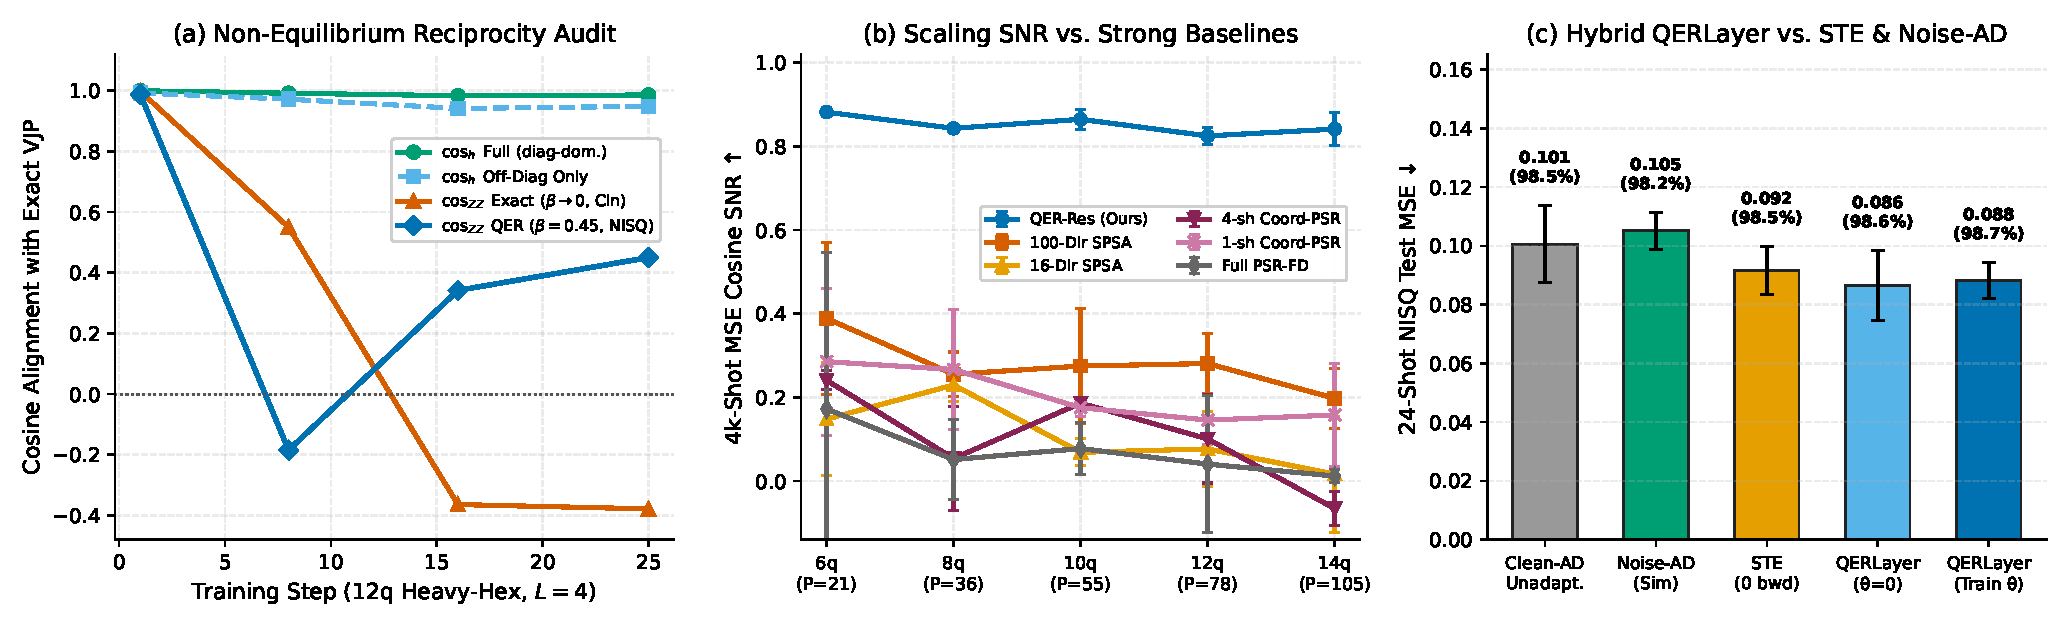
\includegraphics[width=0.98\linewidth]{analysis/fig_reciprocity_scaling.pdf}
\caption{\textbf{Exact $\beta{\to}0$ Reciprocity Audit, Parameter-Scaling Shot SNR, and Hybrid \texttt{STE} Controls ($3$ Seeds).} (a) On trained $12$q Heavy-Hex ($L{=}4$, Table~\ref{tab:exact_recip}), strictly off-diagonal visible-field reciprocity stays $+0.942$--$+0.993$, whereas $ZZ$ coupler alignment starts at $+0.998$ (Step~$1$), undergoes a transient cubic phase inversion at Step~$8$ ($\beta{=}0.45$: $-0.185$ NISQ), and recovers to $+0.450$ at Step~$25$ under NISQ $\beta{=}0.45$ (vs.\ $-0.379$ clean $\beta{\to}0$). (b) $4{,}000$-shot MSE cosine SNR across $n{=}6{\to}14$ qubits ($P{=}21{\to}105$, Table~\ref{tab:scaling_strong}). (c) $8$q $24$-shot hybrid \texttt{QERLayer} vs.\ $0$-backward-shot \texttt{STE} and offline \texttt{Exact-AD} (Table~\ref{tab:hybrid_ste}).}
\label{fig:reciprocity_scaling_ctrl}
\end{figure}

\subsection{When Does Reciprocity Hold? (\texorpdfstring{$h$}{h}-Block vs.\ \texorpdfstring{$ZZ$}{ZZ}-Block and Step-8 Inversion)}
\label{sec:mech}
To test Proposition~\ref{prop:centered_bias} quantitatively, we audited exact $\beta{\to}0$ Jacobians, finite-$\beta$ contrastive updates, and $3$-seed MSE gradient decompositions across random initializations and trained $L{=}2$ and $L{=}4$ checkpoints (Figure~\ref{fig:reciprocity_scaling_ctrl}(a), Table~\ref{tab:exact_recip}).

\begin{table}[t!]
\centering
\caption{\textbf{Microscopic Non-Equilibrium Reciprocity Audit Across Random Draws, Trained $12$q Heavy-Hex ($L{=}4$), and $3$-Seed MSE Decomposition.} Top: exact $\beta{\to}0$ diagonal fraction of $J_h[i,j]{=}\partial\langle Z_i\rangle/\partial h_j$, full vs.\ strictly off-diagonal visible-field cosine $\cos_h$, and $ZZ$ coupler alignment $\cos_{ZZ}$ at $\beta{\to}0$ vs.\ $\beta{=}0.45$ (Clean / NISQ). Bottom: $3$-seed $12$q comparison of $2$-circuit \texttt{QER-Grad} vs.\ $3$-circuit \texttt{QER-Res} against exact $-\nabla_\theta\mathcal{L}_{\text{MSE}}$.}
\label{tab:exact_recip}
\small
\resizebox{\textwidth}{!}{%
\begin{tabular}{@{}lcccc@{}}
\toprule
\textbf{Regime / Checkpoint} & \textbf{Diag.\ Frac.\ $h$} & $\cos_h$ (Full / Off-Diag) & $\cos_{ZZ}^{\beta\to 0}$ (Clean / NISQ) & $\cos_{ZZ}^{\beta=0.45}$ (Clean / NISQ) \\
\midrule
Random $L{=}1$: \texttt{rand\_0.2} / \texttt{rand\_1.0} ($10$q) & $1.000$ / $1.000$ & $+1.000$ / $+0.000$ & $+0.783$ / $+0.778$ \ ($0.978$/$0.978$) & $+0.810$ / $+0.804$ \ ($0.983$/$0.982$) \\
Random $L{=}2$: \texttt{rand\_0.2} / \texttt{rand\_0.6} ($10$q) & $0.998$ / $0.986$ & $+1.000$ / $+0.985$ ($+0.951$) & $+0.803$ / $+0.813$ \ ($0.880$/$0.876$) & $+0.824$ / $+0.833$ \ ($0.890$/$0.888$) \\
Random $L{=}4$: \texttt{rand\_0.2} / \texttt{rand\_0.6} ($10$q) & $0.980$ / $0.899$ & $+0.999$ / $+0.984$ ($+0.921$) & $+0.925$ / $+0.909$ \ ($0.922$/$0.922$) & $+0.946$ / $+0.932$ \ ($0.930$/$0.931$) \\
\midrule
Trained $12$q Heavy-Hex $L{=}4$, Step 1 ($\max|\theta|{=}0.13$) & $0.993$ & $+1.000$ / $+0.993$ & $+0.998$ / $+0.998$ & $+0.989$ / $+0.988$ \\
Trained $12$q Heavy-Hex $L{=}4$, Step 8 ($\max|\theta|{=}0.89$) & $0.868$ & $+0.992$ / $+0.972$ & $+0.550$ / $+0.515$ & $-0.254$ / $-0.185$ \\
Trained $12$q Heavy-Hex $L{=}4$, Step 16 ($\max|\theta|{=}1.11$) & $0.844$ & $+0.983$ / $+0.942$ & $-0.364$ / $-0.095$ & $+0.048$ / $+0.342$ \\
Trained $12$q Heavy-Hex $L{=}4$, Step 25 ($\max|\theta|{=}1.09$) & $0.847$ & $+0.986$ / $+0.949$ & $-0.379$ / $-0.090$ & $+0.137$ / $+0.450$ \\
\midrule
\textbf{$3$-Seed $12$q $L{=}2$ MSE Alignment vs.\ Step} & \textbf{$t{=}1$} & \textbf{$t{=}25$} & \textbf{$t{=}50$} & \textbf{$t{=}100$ / $t{=}200$} \\
\midrule
$2$-Ckt \texttt{QER-Grad} vs.\ $\nabla_\theta\mathbb{E}[\mathbf{x}_0^\top\mathbf{z}]$ ($ZZ$, Clean) & $+0.995 \pm 0.000$ & $+0.745 \pm 0.082$ & $+0.751 \pm 0.052$ & $+0.574 \pm 0.092$ / $+0.378 \pm 0.240$ \\
$2$-Ckt \texttt{QER-Grad} vs.\ $-\nabla_\theta\mathcal{L}_{\text{MSE}}$ ($ZZ$, Clean) & $+0.811 \pm 0.023$ & $-0.200 \pm 0.059$ & $-0.288 \pm 0.115$ & $-0.146 \pm 0.218$ / $+0.315 \pm 0.047$ \\
\textbf{$3$-Ckt \texttt{QER-Res} vs.\ $-\nabla_\theta\mathcal{L}_{\text{MSE}}$ ($ZZ$, Clean)} & $\mathbf{+0.994 \pm 0.001}$ & $\mathbf{+0.494 \pm 0.085}$ & $\mathbf{+0.472 \pm 0.041}$ & $\mathbf{+0.404 \pm 0.019}$ / $\mathbf{+0.404 \pm 0.026}$ \\
\textbf{$3$-Ckt \texttt{QER-Res} vs.\ $-\nabla_\theta\mathcal{L}_{\text{MSE}}$ ($ZZ$, NISQ)} & $\mathbf{+0.991 \pm 0.001}$ & $\mathbf{+0.635 \pm 0.057}$ & $\mathbf{+0.519 \pm 0.054}$ & $\mathbf{+0.502 \pm 0.040}$ / $\mathbf{+0.574 \pm 0.043}$ \\
\bottomrule
\end{tabular}%
}
\end{table}

Table~\ref{tab:exact_recip} establishes four mechanistic properties:
\begin{enumerate}[leftmargin=1.4em,itemsep=2pt,topsep=2pt]
  \item \textbf{Off-Diagonal Visible-Field Reciprocity:} Across all depths and checkpoints, full visible-field alignment satisfies $\cos(\text{JVP},\text{VJP})_h \ge 0.983$. Separating diagonal entries ($J_{ii}\equiv J_{ii}^\top$) from off-diagonal cross-field couplings confirms that at $L{=}1$, the diagonal fraction is identically $1.000$ and off-diagonal $\cos_h{=}0.000$, matching Proposition~\ref{prop:centered_bias} ($\partial\langle Z_1\rangle/\partial h_2\equiv 0$) to machine precision. On trained $12$q Heavy-Hex ($L{=}4$), however, as the diagonal fraction drops to $0.844$--$0.847$, the \emph{strictly off-diagonal} cosine remains $+0.942$--$+0.993$, confirming genuine multi-qubit visible-field reciprocity for $L\ge 2$.
  \item \textbf{Why $3$-Circuit \texttt{QER-Res} Is Essential for $ZZ$ Couplers:} In the bottom panel of Table~\ref{tab:exact_recip}, $2$-circuit target nudging (\texttt{QER-Grad}) stays positively aligned with the correlation gradient $\nabla_\theta\mathbb{E}[\mathbf{x}_0^\top\mathbf{z}]$ ($+0.378$ to $+0.995$), but turns \emph{negative} against the true MSE gradient $-\nabla_\theta\mathcal{L}_{\text{MSE}}$ mid-training ($-0.200$ at $t{=}25$, $-0.288$ at $t{=}50$) because it omits $-\frac{1}{2}\nabla_\theta\|\mathbf{z}\|^2$. Switching to $3$-circuit residual nudging (\texttt{QER-Res}) restores positive $ZZ$ MSE alignment at every step ($+0.404$--$+0.994$ Clean; $+0.502$--$+0.991$ NISQ).
  \item \textbf{Transient Step-$8$ Finite-$\beta$ Inversion:} On $L{=}4$ Heavy-Hex (Table~\ref{tab:exact_recip}, middle), $ZZ$ alignment starts at $+0.998$ at Step~$1$ ($\max|\theta|{=}0.13$, deep inside the small-$|\boldsymbol{\theta}|$ Kubo regime). At Step~$8$ ($\max|\theta|{=}0.89$), exact $\beta{\to}0$ alignment is still positive ($+0.550$ Clean / $+0.515$ NISQ; $+0.475 / +0.450$ at $\beta{=}0.10$), yet $\beta{=}0.45$ briefly flips negative ($-0.254$ Clean / $-0.185$ NISQ). At this intermediate weight scale, accumulated $4$-layer nudge phases ($\sim 4\beta g_\ell \gtrsim \pi/2$) cause the third-order cubic curvature term $\frac{\beta^2}{6} D_{\mathbf{y}}^3\langle Z_u Z_v\rangle$ to briefly dominate just before exact $\beta{\to}0$ reciprocity itself crosses zero. Thus finite $\beta$ does \emph{not} guarantee pointwise monotone descent at every step; traversing this band relies on early small-$|\boldsymbol{\theta}|$ sign lock-in (Steps~$1$--$6$), Adam momentum ($\beta_1{=}0.75$), and box clipping.
  \item \textbf{Late-Training Breakdown \& NISQ Phase Smoothing:} By Steps~$16$--$25$ ($\max|\theta|{=}1.09$--$1.11$), exact $\beta{\to}0$ clean $ZZ$ cosine drops to $-0.379$ ($\sim 60^\circ$--$110^\circ$ direction error), rises to $-0.090$ under NISQ depolarization, turns positive ($+0.137$) at clean $\beta{=}0.45$, and reaches $+0.450$ under operational NISQ $\beta{=}0.45$.
\end{enumerate}

\subsection{Parameter-Scaling Shot SNR and Two-Qubit CNOT Noise Robustness}
\label{sec:new_controls}
Having established that \texttt{QER-Res} trades exact VJP reciprocity for simultaneous $\mathcal{O}(1)$-circuit readout, we next test whether its variance reduction outweighs its surrogate bias under realistic finite-shot budgets.

\begin{table}[t!]
\centering
\caption{\textbf{$4{,}000$-Shot MSE Cosine SNR Scaling vs.\ Multi-Direction SPSA and $1$-/$4$-Shot Coordinate PSR ($3$ Seeds, $L{=}2$, All-to-All Ising Circuit).} Cosine similarity between each finite-shot estimator ($4{,}000$ total shots) and the exact noiseless MSE gradient $-\nabla_\theta\mathcal{L}_{\text{MSE}}$.}
\label{tab:scaling_strong}
\small
\resizebox{\textwidth}{!}{%
\begin{tabular}{@{}cccccc@{}}
\toprule
\textbf{Qubits $n$} & \textbf{Params $P$} & \textbf{\texttt{QER-Res} (Ours) $\uparrow$} & \textbf{SPSA ($16$-dir / $100$-dir)} & \textbf{Coord-PSR ($1$-sh / $4$-sh)} & \textbf{Full PSR-FD} \\
\midrule
6  & 21  & $\mathbf{+0.882}$ & $+0.148$ / $+0.389$ & $+0.285$ / $+0.241$ & $+0.172$ \\
8  & 36  & $\mathbf{+0.843}$ & $+0.230$ / $+0.255$ & $+0.267$ / $+0.054$ & $+0.051$ \\
10 & 55  & $\mathbf{+0.865}$ & $+0.069$ / $+0.275$ & $+0.175$ / $+0.186$ & $+0.078$ \\
12 & 78  & $\mathbf{+0.825}$ & $+0.077$ / $+0.281$ & $+0.146$ / $+0.101$ & $+0.041$ \\
14 & 105 & $\mathbf{+0.841}$ & $+0.017$ / $+0.198$ & $+0.158$ / $-0.066$ & $+0.012$ \\
\bottomrule
\end{tabular}%
}
\end{table}

Across $n{=}6{\to}14$ qubits ($P{=}21{\to}105$; Table~\ref{tab:scaling_strong}, Figure~\ref{fig:reciprocity_scaling_ctrl}(b)), \texttt{QER-Res} holds a flat $4{,}000$-shot MSE cosine SNR of \textbf{$+0.882\to +0.841$}, outperforming variance-reduced $100$-direction \texttt{SPSA} ($+0.389\to +0.198$), $1$-shot and $4$-shot randomized-coordinate \texttt{PSR} ($+0.285\to +0.158$ and $+0.241\to -0.066$), $16$-direction \texttt{SPSA} ($+0.148\to +0.017$), and full-sweep \texttt{PSR-FD} ($+0.172\to +0.012$) by $>4\times$ at $14$ qubits.

\begin{figure}[t!]
\centering
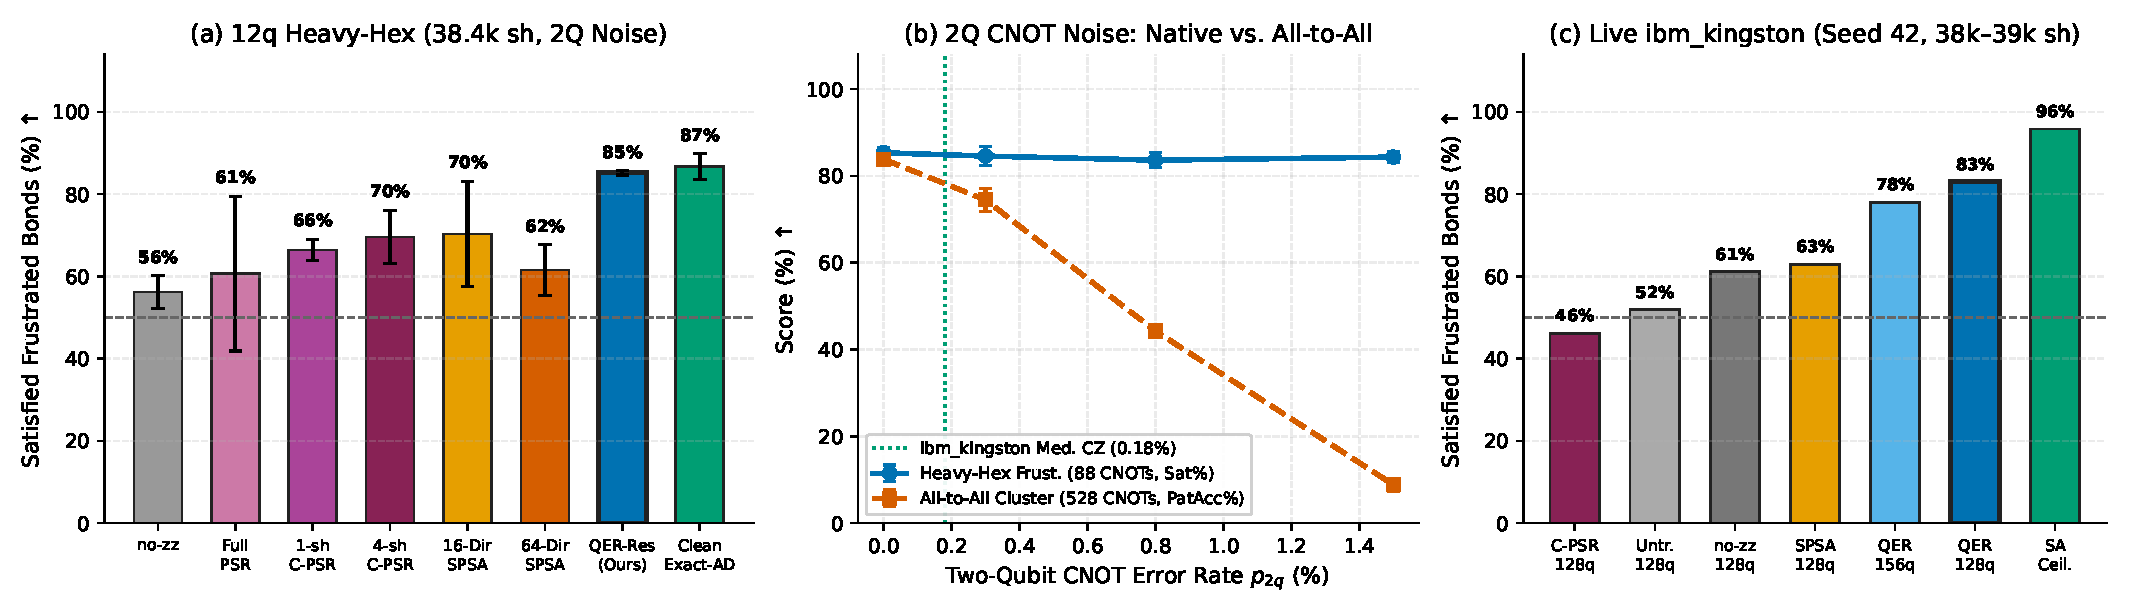
\includegraphics[width=0.98\linewidth]{analysis/fig_heron_spinglass.pdf}
\caption{\textbf{Controlled $3$-Seed $12$q Heavy-Hex Spin-Glass Benchmarks, Two-Qubit CNOT Noise Sweep, and Live \texttt{ibm\_kingston} Breakdown.} (a) $12$q \texttt{FakeKingston} Heavy-Hex ($|E|{=}11, L{=}4, p_{2\text{q}}{=}0.5\%, 38.4\text{k}$ shots; Table~\ref{tab:hw_controls_main}): \texttt{QER-Res} ($85.2\pm 0.5\%$) tracks within $1.5\text{ pp}$ of noiseless \texttt{Exact-AD} ($86.7\pm 3.1\%$). (b) Two-qubit CNOT noise stress sweep ($p_{2\text{q}}\in[0,1.5\%]$; Table~\ref{tab:hw_controls_main}): native Heavy-Hex ($88$ CNOTs) stays flat ($85.3\%{\to}84.3\%$) while All-to-All ($528$ CNOTs) collapses ($83.9\%{\to}8.9\%$). (c) Live \texttt{ibm\_kingston} \texttt{seed=42} summary.}
\label{fig:heron_spinglass_ctrl}
\end{figure}

\begin{table}[t!]
\centering
\caption{\textbf{Controlled $3$-Seed $12$-Qubit Heavy-Hex Frustrated Spin Glass and Two-Qubit CNOT Noise Sweep ($L{=}4$, $38.4\text{k}$ Shots).} Left: shot-matched optimizer comparison on a calibrated $12$q \texttt{FakeKingston} subgraph ($|E|{=}11, P{=}23, 0$ SWAPs) at $p_{\text{depol,2q}}{=}0.5\%, p_{\text{depol}}{=}0.5\%, p_{\text{ro}}{=}1.5\%$. Right: sweeping two-qubit CNOT depolarizing rate $p_{\text{depol,2q}}\in[0,1.5\%]$ on native Heavy-Hex ($88$ CNOTs) vs.\ All-to-All Stride-$3$ ($528$ CNOTs).}
\label{tab:hw_controls_main}
\small
\resizebox{\textwidth}{!}{%
\begin{tabular}{@{}lccc@{\hspace{1.8em}}ccccc@{}}
\toprule
\multicolumn{4}{c}{\textbf{(a) $12$q Heavy-Hex Optimizer Suite ($p_{2\text{q}}{=}0.5\%$)} } & \multicolumn{5}{c}{\textbf{(b) Two-Qubit CNOT Noise Sweep ($88$ vs.\ $528$ CNOTs)}} \\
\cmidrule(r){1-4}\cmidrule(l){5-9}
\textbf{Optimizer / Control} & \textbf{Sat.\ Bonds $\uparrow$} & \textbf{Gap $\uparrow$} & \textbf{Mean $E$ $\downarrow$} & $p_{\text{depol,2q}}$ & \textbf{HH Sat.\ $\uparrow$} & \textbf{HH Gap $\uparrow$} & \textbf{All2All Acc $\uparrow$} & \textbf{All2All Corr $\uparrow$} \\
\midrule
Untrained QPU ($\theta{=}0$) & $50.3 \pm 0.5\%$ & $0.0 \pm 0.0\%$ & $-0.07$ & $0.0\%$ & $85.3 \pm 1.1\%$ & $74.1 \pm 2.0\%$ & $83.9 \pm 1.5\%$ & $+0.820$ \\
\texttt{QER no-zz} ($0$ $ZZ$) & $56.2 \pm 3.9\%$ & $12.2 \pm 9.1\%$ & $-1.36$ & $0.3\%$ & $84.6 \pm 2.3\%$ & $72.5 \pm 4.1\%$ & $74.5 \pm 2.7\%$ & $+0.797$ \\
Full-Sweep \texttt{PSR-FD} & $60.7 \pm 18.8\%$ & $22.7 \pm 39.8\%$ & $-2.35$ & $0.8\%$ & $83.6 \pm 1.8\%$ & $70.5 \pm 3.3\%$ & $44.3 \pm 1.5\%$ & $+0.593$ \\
High-Dir \texttt{SPSA} ($64$-dir) & $61.6 \pm 6.1\%$ & $23.9 \pm 12.5\%$ & $-2.54$ & $1.5\%$ & $84.3 \pm 1.2\%$ & $72.0 \pm 1.8\%$ & $8.9 \pm 1.5\%$ & $+0.255$ \\
$1$-Shot \texttt{Coord-PSR}~\cite{sweke2020sgd} & $66.4 \pm 2.6\%$ & $33.9 \pm 5.9\%$ & $-3.61$ & \multicolumn{5}{l}{} \\
$4$-Shot \texttt{Coord-PSR}~\cite{sweke2020sgd} & $69.6 \pm 6.5\%$ & $40.9 \pm 13.6\%$ & $-4.31$ & \multicolumn{5}{l}{\scriptsize \textit{Takeaway:} Native Heavy-Hex routing ($0$ SWAPs, $88$ CNOTs)} \\
Multi-Dir \texttt{SPSA} ($16$-dir) & $70.3 \pm 12.8\%$ & $42.7 \pm 27.2\%$ & $-4.47$ & \multicolumn{5}{l}{\scriptsize loses only $-1.0\text{ pp}$ across $p_{2\text{q}}\in[0,1.5\%]$ ($>8\times$ Kingston's} \\
\texttt{Adam-QER} ($2$-ckt) & $76.5 \pm 2.2\%$ & $55.3 \pm 4.7\%$ & $-5.83$ & \multicolumn{5}{l}{\scriptsize $0.18\%$ median CZ error), whereas $528$-CNOT all-to-all} \\
\textbf{\texttt{QER-Res} (Ours, $3$-ckt)} & $\mathbf{85.2 \pm 0.5\%}$ & $\mathbf{73.6 \pm 0.6\%}$ & $\mathbf{-7.74}$ & \multicolumn{5}{l}{\scriptsize circuits collapse by $-75.0\text{ pp}$ ($83.9\%{\to}8.9\%$).} \\
\textit{Ref: Clean \texttt{Exact-AD}} & $86.7 \pm 3.1\%$ & $77.0 \pm 6.8\%$ & $-8.08$ & \multicolumn{5}{l}{} \\
\textit{Ref: SA Ceiling} & $97.7 \pm 0.5\%$ & $100.0 \pm 0.0\%$ & $-10.49$ & \multicolumn{5}{l}{} \\
\bottomrule
\end{tabular}%
}
\end{table}

Table~\ref{tab:hw_controls_main} and Figure~\ref{fig:heron_spinglass_ctrl} test end-to-end training on a $3$-seed $12$-qubit \texttt{FakeKingston} Heavy-Hex frustrated spin glass ($|E|{=}11, L{=}4, 38.4\text{k}$ shots) under explicit two-qubit CNOT noise ($p_{\text{depol,2q}}{=}0.5\%$). Under identical shots and noise, $3$-circuit \texttt{QER-Res} reaches \textbf{$85.2\pm 0.5\%$ satisfied bonds} ($73.6\pm 0.6\%$ gap closed), tracking within $1.5\text{ pp}$ of noiseless \texttt{Exact-AD} ($86.7\pm 3.1\%$) with $6\times$ lower seed variance, and outperforming $2$-circuit \texttt{Adam-QER} ($76.5\%$), $16$-direction \texttt{SPSA} ($70.3\%$), $4$-shot and $1$-shot sparse-Adam \texttt{Coord-PSR} ($69.6\%$ and $66.4\%$), $64$-direction \texttt{SPSA} ($61.6\%$; at small $P{=}23$, $12$-shot per-circuit noise outweighs mask-crosstalk reduction), full-sweep \texttt{PSR-FD} ($60.7\%$), and uncoupled \texttt{no-zz} ($56.2\%$). Sweeping $p_{\text{depol,2q}}$ from $0.0\%{\to}1.5\%$ (Table~\ref{tab:hw_controls_main}(b)) shows that native Heavy-Hex ($88$ CNOTs, $0$ SWAPs) stays virtually flat ($85.3\%{\to}84.3\%$), whereas all-to-all coupling ($528$ CNOTs) collapses from $83.9\%{\to}8.9\%$.

\subsection{Zero-Shortcut Multi-Qubit \texorpdfstring{$ZZ$}{ZZ} Attribution and Hybrid \texttt{QERLayer} Controls}
\label{sec:hybrid_sim}
To verify multi-qubit $ZZ$ learning beyond sparse spin glasses while eliminating classical conditioning shortcuts, Table~\ref{tab:quantum_attribution} evaluates three $12$--$14$-qubit benchmarks where $W_{\text{cond}}\mathbf{c}$ is either deleted ($0$ classical weights) or tested without BatchNorm whitening:

\begin{table}[t!]
\centering
\caption{\textbf{Controlled Zero-Shortcut $ZZ$ Attribution ($3$ Seeds, NISQ $3.5\%/4\%$ Unless Marked Clean).} Removing $W_{\text{cond}}\mathbf{c}$ ($12$q Stride-$3$ Cluster and $13$--$14$q Label Qubits) or disabling \texttt{BatchNorm1d} isolates two-qubit $ZZ$ learning relative to same-circuit \texttt{Exact-AD} and \texttt{ClassicalIsing-EP}.}
\label{tab:quantum_attribution}
\small
\resizebox{\textwidth}{!}{%
\begin{tabular}{@{}llccccc@{}}
\toprule
\textbf{Benchmark} & \textbf{Method / Variant} & \textbf{Params} & \textbf{Primary Acc $\uparrow$} & \textbf{Structure / FID} & \textbf{Cov / 10-Way} & \textbf{RMSE / Prec} \\
\midrule
\multirow{6}{*}{\shortstack[l]{Zero-AE $12$q Stride-$3$\\Correlated Cluster\\($\mathbf{c}=\mathbf{0}$, $L{=}4$, $40\text{k}$ sh)}} & \texttt{QER no-zz} / \texttt{chain} / \texttt{grid4} & $12$--$29$ & $1.4 \pm 0.5\%$ & $\text{Corr}=+0.001$ & $\text{ModeCov}=16.7\%$ & $\text{RMSE}=0.524$ \\
 & \texttt{Adam-SPSA} ($L{=}4$, FwdOLS, NISQ) & $78$ & $11.9 \pm 13.2\%$ & $\text{Corr}=+0.030$ & $\text{ModeCov}=8.3\%$ & $\text{RMSE}=0.515$ \\
 & \textbf{\texttt{QER-Res} ($3$-ckt MSE, $L{=}4$, NISQ)} & $78$ & $74.8 \pm 4.3\%$ & $+0.688 \pm 0.076$ & $\mathbf{100.0 \pm 0.0\%}$ & $0.205$ \\
 & \textbf{\texttt{Adam-QER} ($2$-ckt, $L{=}4$, NISQ / Clean)} & $78$ & $80.2$ / $89.3\%$ & $+0.569$ / $+0.687$ & $87.5$ / $\mathbf{100.0\%}$ & $0.266$ / $0.207$ \\
 & \textit{Ref: \texttt{Exact-AD} ($L{=}4$, FwdOLS, Clean)} & $78$ & $94.5 \pm 1.2\%$ & $+0.890 \pm 0.051$ & $100.0 \pm 0.0\%$ & $0.112$ \\
 & \textit{Ref: \texttt{ClassicalIsing-EP} (Float64 Attr.)} & $78$ & $100.0 \pm 0.0\%$ & $+0.939 \pm 0.066$ & $75.0 \pm 35.4\%$ & $0.357$ \\
\midrule
\multirow{3}{*}{\shortstack[l]{Zero-$W_{\text{cond}}$ $13$q $\{0,1\}$\\($L{=}3, 80\text{k}$ sh)}} & \texttt{no-zz} / Tuned SPSA / \texttt{iCANS-PSR} & $13$--$91$ & $49.9$ / $50.0$ / $49.6\%$ & -- & $2.4 / 0.0 / 0.0\%$ & -- \\
 & \textbf{\texttt{Adam-QER all} (NISQ)} & $91$ & $\mathbf{99.3 \pm 0.2\%}$ & -- & $2.9 \pm 2.1\%$ {\scriptsize(10-way)} & -- \\
 & \textit{Ref: Same-Circuit \texttt{Exact-AD} (Clean)} & $91$ & $100.0\%$ & -- & $98.2\%$ {\scriptsize(10-way)} & -- \\
\midrule
\multirow{3}{*}{\shortstack[l]{Zero-$W_{\text{cond}}$ $14$q $\{0,1,4\}$\\($L{=}3, 80\text{k}$ sh)}} & \texttt{QER no-zz} (NISQ) & $14$ & $33.1 \pm 1.8\%$ & -- & $23.3\%$ {\scriptsize(10-way)} & -- \\
 & \textbf{\texttt{Adam-QER all} (NISQ)} & $105$ & $\mathbf{71.0 \pm 16.0\%}$ & -- & $59.3 \pm 9.6\%$ {\scriptsize(10-way)} & -- \\
 & \textit{Ref: Same-Circuit \texttt{Exact-AD} (Clean)} & $105$ & $100.0\%$ & -- & $96.7\%$ {\scriptsize(10-way)} & -- \\
\midrule
\multirow{2}{*}{\shortstack[l]{Unwhitened Fashion\\(\texttt{bn=False}, $80\text{k}$ sh)}} & \texttt{QER no-zz}$^\dagger$ ($12{+}2$q, NISQ) & $158$ & $71.7 \pm 0.9\%$ & $\text{CondLatFID}=2.28$ & $\text{FeatFID}=113.5$ & $\text{Prec}=0.982$ \\
 & \textbf{\texttt{Adam-QER Full} ($ZZ$, NISQ)} & $224$ & $73.1 \pm 3.1\%$ & $\mathbf{1.79 \pm 0.07}$ & $\mathbf{99.3 \pm 4.4}$ & $\mathbf{0.994}$ \\
\bottomrule
\multicolumn{7}{l}{\scriptsize $^\dagger$Fashion \texttt{no-zz} ($158$p) removes all $66$ visible--visible $ZZ$ couplings while retaining $24$ visible--hidden ancilla edges ($120\ W_{\text{cond}} + 14\ b + 24\ J_{vh}$).}
\end{tabular}%
}
\end{table}

\begin{itemize}[leftmargin=1.4em,itemsep=2pt,topsep=2pt]
  \item \textbf{Autoencoder-Free $12$q Stride-$3$ Correlated Cluster ($\mathbf{c}{=}\mathbf{0}$):} The target distribution comprises the $8$ discrete modes $\mathbf{x}_m[q] = s_{q\bmod 3}$ ($s_0,s_1,s_2\in\{\pm 1\}$)—three disjoint $4$-qubit ferromagnetic cliques with exact zero single-qubit marginals ($\mathbb{E}[x_i]{=}0$) and non-local stride-$3$ couplings. Uncoupled or local topologies (\texttt{no-zz}, \texttt{chain}, \texttt{grid4}) cannot express stride-$3$ correlations ($1.4\%$ pattern accuracy), and equal-shot \texttt{SPSA} stalls at $11.9\%$. At $L{=}4$ with forward-OLS sharpening, $3$-circuit \texttt{QER-Res} reaches $+0.688\pm 0.076$ intra-cluster correlation, \textbf{$100.0\pm 0.0\%$ mode coverage} (all $8/8$ modes), and $74.8\pm 4.3\%$ exact pattern accuracy ($80.2\%$ for $2$-circuit \texttt{Adam-QER}), recovering $80\%$--$85\%$ of noiseless \texttt{Exact-AD} ($94.5\%$; noiseless float64 \texttt{ClassicalIsing-EP} reaches $100.0\%$ accuracy at $75.0\%$ mode coverage).
  \item \textbf{Zero-$W_{\text{cond}}$ Label-Qubit Routing ($13$--$14$q) \& Unwhitened Fashion:} Deleting $W_{\text{cond}}$ completely and injecting class codes only as fixed $\pm 1.15$ fields on $1$--$2$ unnudged ancilla qubits ($L{=}3$, uncalibrated readout) forces class information to travel exclusively through $ZZ$ couplers. While \texttt{no-zz}, tuned \texttt{SPSA}, and \texttt{iCANS-PSR} remain at chance ($49.6\%$--$50.0\%$ on $13$q $\{0,1\}$; $33.1\%$ on $14$q $\{0,1,4\}$), \texttt{Adam-QER} lifts $2$-way subset accuracy to $99.3\pm 0.2\%$ on $13$q and $3$-way accuracy to $71.0\pm 16.0\%$ on $14$q ($59.3\%$ $10$-way). \emph{Candid caveat:} on $13$q $\{0,1\}$, $10$-way accuracy is only $2.9\pm 2.1\%$ (vs.\ $98.2\%$ clean \texttt{Exact-AD}) because uncalibrated $L{=}3$ depolarizing attenuation shrinks latent amplitudes toward the origin where the evaluator assigns out-of-subset classes. On unwhitened Fashion-MNIST (\texttt{bn=False}), adding visible $ZZ$ couplers lowers \texttt{CondLatFID} ($2.28{\to}1.79$) and \texttt{FeatFID} ($113.5{\to}99.3$), though \texttt{ClfAcc} ($73.1\%$ vs.\ $71.7\%$) is within $1\sigma$.
\end{itemize}

\begin{table}[t!]
\centering
\caption{\textbf{End-to-End Hybrid \texttt{QERLayer} Controls ($3$ Seeds).} Left: $8$-qubit $24$-shot NISQ regression comparing \texttt{QERLayer} against $0$-backward-shot \texttt{STE} and offline Clean/Noise-Aware \texttt{Exact-AD}. Right: $12$-qubit MNIST hybrid ResMLP scaling ($N{=}2{,}000$, $1.38\text{M}$ QPU shots where shot-based) against equal-shot layered PSR and $6$-shot classical Binomial noise.}
\label{tab:hybrid_ste}
\small
\resizebox{\textwidth}{!}{%
\begin{tabular}{@{}lccc@{\hspace{1.6em}}lcccc@{}}
\toprule
\multicolumn{4}{c}{\textbf{(a) $8$q $24$-Shot NISQ Hybrid Control Suite}} & \multicolumn{5}{c}{\textbf{(b) $12$q Hybrid ResMLP Scaling ($h{=}48, \sigma{=}0.35 / 0.85$)}} \\
\cmidrule(r){1-4}\cmidrule(l){5-9}
\textbf{Training Rule} & \textbf{Bwd Shots} & \textbf{Test MSE $\downarrow$} & \textbf{Sign Acc $\uparrow$} & \textbf{Hybrid Model / Control} & \textbf{ClfAcc (\%) $\uparrow$} & \textbf{FeatFID $\downarrow$} & \textbf{Prec $\uparrow$} & \textbf{Rec $\uparrow$} \\
\midrule
Clean \texttt{Exact-AD} $\to$ NISQ24 & $0$ (Sim) & $0.1006 \pm 0.0132$ & $98.5 \pm 0.5\%$ & \texttt{ExactAD-h48} (Clean Eval, $\sigma{=}.85$) & $99.8$ & $94.8$ & $0.996$ & $0.067$ \\
Noise-Aware \texttt{Exact-AD} (Sim) & $0$ (Sim) & $0.1051 \pm 0.0063$ & $98.2 \pm 0.3\%$ & \texttt{ExactAD-h48} ($\to$ NISQ24 Eval) & $88.5$ / $81.4$ & $120.7$ / $151.7$ & $.960 / .942$ & $.308 / .403$ \\
\texttt{STE} ($0$ bwd QPU shots) & $0$ ($1/3\times$ tot) & $0.0917 \pm 0.0082$ & $98.5 \pm 0.3\%$ & \texttt{HybridPSR-h48} ($24$sh, $18$ st) & $35.4$ / $25.9$ & $315.1$ / $275.7$ & $.904 / .888$ & $.360 / .485$ \\
\texttt{QERLayer} ($\theta{=}0$ frozen) & $2$ ckts/samp & $0.0865 \pm 0.0119$ & $98.6 \pm 0.5\%$ & \texttt{HybridPSR-h48} ($4$sh, $100$ st) & $88.8$ / $76.1$ & $108.0$ / $139.3$ & $.955 / .925$ & $.320 / .431$ \\
\textbf{\texttt{QERLayer} (Trainable $\theta$)} & $2$ ckts/samp & $\mathbf{0.0882 \pm 0.0061}$ & $\mathbf{98.7 \pm 0.3\%}$ & \textbf{\texttt{HybridQER-h48} (\texttt{QERLayer})} & $\mathbf{95.5}$ / $\mathbf{89.7}$ & $\mathbf{72.0}$ / $89.5$ & $.976 / .961$ & $.326 / .428$ \\
\multicolumn{4}{l}{} & \texttt{ClassicalResMLP+6shNoise} ($\sigma{=}.85$) & $89.6$ & $\mathbf{70.4}$ & $0.953$ & $\mathbf{0.540}$ \\
\bottomrule
\end{tabular}%
}
\end{table}

\begin{figure}[t!]
\centering
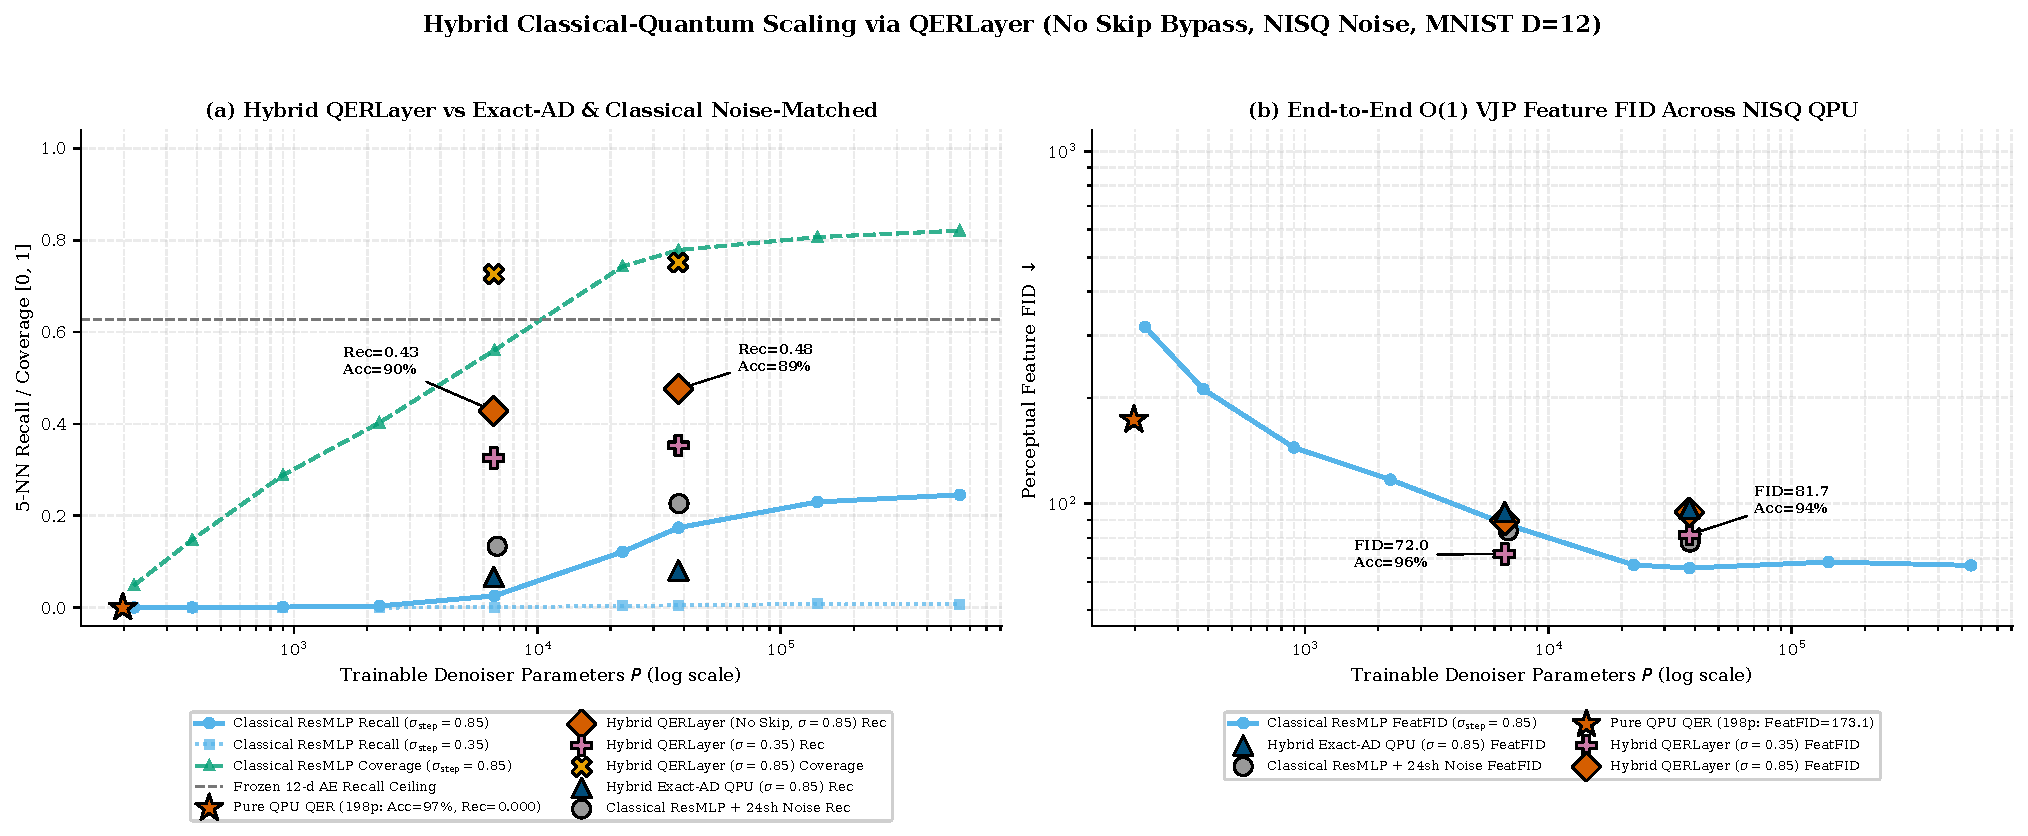
\includegraphics[width=0.82\linewidth]{analysis/fig_hybrid_qpu_diversity.pdf}
\caption{\textbf{End-to-End Hybrid Scaling via \texttt{QERLayer} ($3$ Seeds, $N{=}2{,}000$).} Hardware-in-the-loop surrogate differentiation recovers the $7.0$--$9.4\text{ pp}$ accuracy drop and $+48.7$ to $+71.7$ \texttt{FeatFID} degradation suffered by unadapted clean-trained \texttt{ExactAD} under $24$-shot NISQ deployment, while matched $6$-shot classical Binomial noise confirms stochastic measurement regularization drives sample diversity.}
\label{fig:hybrid_qpu_diversity}
\end{figure}

\paragraph{Hybrid \texttt{QERLayer} vs.\ $0$-Backward-Shot \texttt{STE} and Classical Shot Noise.}
Table~\ref{tab:hybrid_ste} and Figure~\ref{fig:hybrid_qpu_diversity} evaluate Proposition~\ref{prop:vjp} when a classical neural trunk feeds into a noisy quantum layer. On $12$q MNIST hybrid ResMLPs ($h\in\{48,128\}$, $1.38\text{M}$ total shots, $24$ shots/step), deploying an offline clean-trained \texttt{ExactAD} trunk onto $24$-shot noisy hardware drops accuracy by $7.0$--$9.4\text{ pp}$ and degrades \texttt{FeatFID} by $+48.7$ to $+71.7$ compared to end-to-end \texttt{QERLayer} adaptation ($95.5\% / 89.7\%$ vs.\ $88.5\% / 81.4\%$), while equal-shot layered PSR across the $12$ input fields trails by $6.7$--$13.6\text{ pp}$. Two negative controls bound this result honestly: (i) on our $8$q $24$-shot hybrid control suite (Table~\ref{tab:hybrid_ste}(a)), while \texttt{QERLayer} achieves the lowest mean test MSE ($0.0865\pm 0.0119$ frozen $\boldsymbol{\theta}$; $0.0882\pm 0.0061$ jointly trained $\boldsymbol{\theta}$), a $0$-backward-shot Straight-Through Estimator (\texttt{STE}) reaches $0.0917\pm 0.0082$ at $1/3\times$ the QPU shot cost (within $\sim 0.5\sigma$), making \texttt{STE} a strong low-shot alternative whenever $\boldsymbol{\theta}$ is frozen; and (ii) replacing the quantum layer with classical $6$-shot Binomial noise matches or beats hybrid diversity ($89.6\%$ accuracy, $\text{FeatFID}{=}70.4, \text{Rec}{=}0.540$), proving that measurement stochasticity rather than quantum entanglement drives hybrid diversity gains.

% ==============================================================================
\section{Scaling to Live 128--156-Qubit IBM Heron R2 Hardware}
\label{sec:heron}
% ==============================================================================
Equipped with the $12$-qubit verification that native Heavy-Hex routing ($0$ SWAPs) keeps \texttt{QER-Res} flat up to $p_{2\text{q}}{=}1.5\%$ CNOT error, we scale past the $\sim 26$-qubit exact $2^N$ statevector simulation wall onto $128$-qubit noise-pruned subgraphs and the full $156$-qubit chip of IBM's Heron R2 processor \texttt{ibm\_kingston} via Qiskit Runtime \texttt{SamplerV2} batched PUB jobs.

\begin{figure}[t!]
\centering
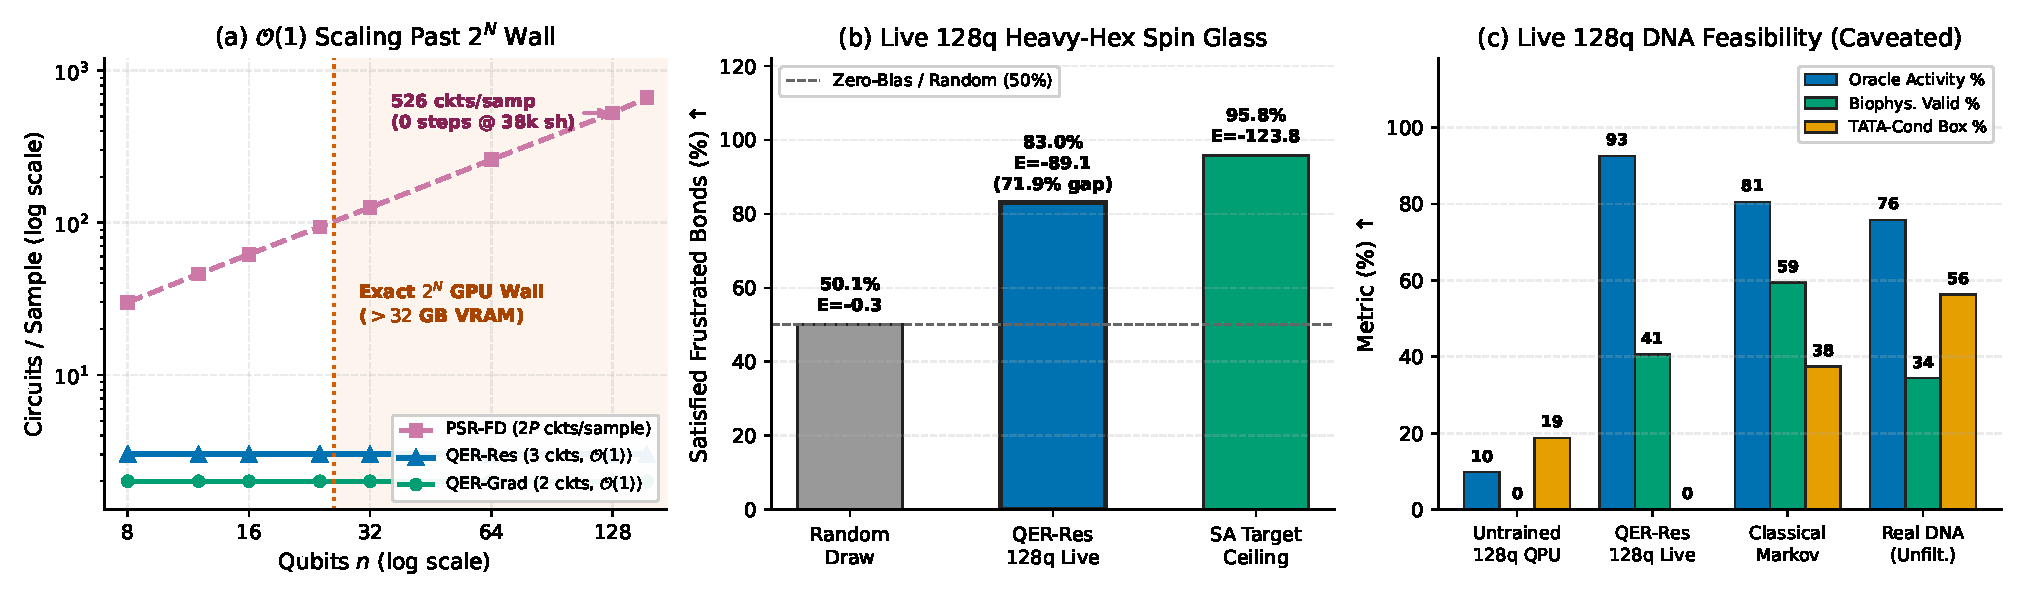
\includegraphics[width=\textwidth]{analysis/fig_heron_live_128q.pdf}
\caption{\textbf{Live $128$--$156$-Qubit IBM Heron R2 (\texttt{ibm\_kingston}) Validation Past the $2^N$ GPU Wall ($0$ SWAPs).} (a) \texttt{QER} uses $2$--$3$ circuits/sample independent of $n$, whereas PSR scales as $2P$ ($664$ circuits/sample at $156$q, $0$ steps inside $38\text{k}$ shots). (b) On genuinely frustrated $\pm J$ Heavy-Hex spin glasses ($\mathbb{E}[x_i]{=}0$), raw live \texttt{QER-Res} reaches $83.0\%$ (\texttt{seed=42}, $\circ$) and $87.7\%$ (\texttt{seed=43}, $\blacklozenge$; two-instance mean $85.3\%$) satisfied bonds, and $78.0\%$ on the unpruned full $156$-qubit chip, outperforming live $128$q \texttt{Coord-PSR} ($46.1\%$), \texttt{no-zz} ($61.1\%$), and $96$-direction \texttt{SPSA} ($62.9\%$ / $49.1\%$, mean $56.0\%$; see Table~\ref{tab:heron_gen_audit} for raw sector-locking vs.\ $77.8\%$ batch-debiased evaluation). (c) Live $128$q ($64\text{ bp}$) Fixed-TATA DNA controls show \texttt{QER-Res} ($75\%$ activity, $53\%$ valid, $75\%$ TATA) outperforming equal-shot live Chain-Rule \texttt{SPSA} ($47\% / 31\% / 62\%$), while live \texttt{no-zz} ($82\% / 59\% / 88\%$) candidly isolates $1$-body positional dominance on DNA.}
\label{fig:heron_live}
\end{figure}

\subsection{Calibration Audit, Zero-SWAP Subgraph Routing, and Readout Mitigation}
\label{sec:heron_cal}
Auditing all three $156$-qubit IBM Heron R2 processors (Table~\ref{tab:heron_audit}) reveals heavy-tailed error distributions: full $156$-qubit layouts contain $8$--$19$ qubits with $>5\%$ readout error and $22$--$40$ couplers with $>2\%$ CZ error. Greedily selecting a connected $128$-qubit subgraph on \texttt{ibm\_kingston} ($|E|{=}135$ native Heavy-Hex edges, $4$ edge colors for parallel $R_{ZZ}$ execution, $0$ SWAP gates) eliminates every $>5\%$ readout outlier (\texttt{RO}$>5\%$: $16{\to}0$, median $1.03\%$) and reduces $>2\%$ couplers from $24{\to}3$ (median CZ error $0.18\%$, $T_1{=}283\,\mu\text{s}, T_2{=}144\,\mu\text{s}$). Before training, a single $2$-circuit all-$|0\rangle$/all-$|1\rangle$ job ($512$ shots, accounted outside the training budget) fits per-qubit marginal readout offsets and scales $(\text{offset}_i, \text{scale}_i)$, inverted on CPU at zero extra shot cost alongside inverse-OLS gain calibration ($\text{gain}\in[0.40,1.00]$). At $128$ qubits ($P{=}263$), packing $M{=}24$ samples $\times 48$ shots into batched PUBs executes $11$ \texttt{QER-Res} updates in $38{,}016$ training shots ($9.8\,$s pure pulse time at $4{,}000$ shots/s; evaluation draws $T{=}4{\times}N{=}32{\times}96{=}12{,}288$ shots per model, accounted separately). Against layer-tied finite-difference PSR ($2P{=}526$ circuits/sample—a conservative baseline compared to exact analytic PSR's $2LP{=}2{,}104$ circuits/sample at $L{=}4$), $3$-circuit \texttt{QER-Res} achieves a \textbf{$175\times$ circuit compression} ($526/3$; \textbf{$263\times$} for $2$-circuit \texttt{QER-Grad}); at $156$ qubits ($P{=}332$), compression reaches \textbf{$221\times$} for \texttt{QER-Res} ($664/3$) and \textbf{$332\times$} for \texttt{QER-Grad}.

\begin{table}[t!]
\centering
\caption{\textbf{IBM Heron R2 ($156$q) Calibration Audit and Noise-Pruned $128$q \texttt{ibm\_kingston} Subgraph.} Pruning eliminates all $>5\%$ readout outliers while preserving $0$ SWAP routing overhead.}
\label{tab:heron_audit}
\small
\resizebox{\textwidth}{!}{%
\begin{tabular}{@{}lccccccc@{}}
\toprule
\textbf{Backend / Layout} & \textbf{Edges} & \textbf{Med CZ} & \textbf{p90 CZ} & \textbf{CZ$>$2\%} & \textbf{Med RO} & \textbf{RO$>$5\%} & \textbf{$T_1 / T_2$ ($\mu$s)} \\
\midrule
\texttt{ibm\_marrakesh} ($156$q) & 176 & $0.33\%$ & $4.47\%$ & 40 & $0.95\%$ & 19 & $197 / 118$ \\
\texttt{ibm\_fez} ($156$q)       & 176 & $0.39\%$ & $1.43\%$ & 22 & $0.76\%$ & 8  & $145 / 88$ \\
\texttt{ibm\_kingston} ($156$q)  & 176 & $0.18\%$ & $0.86\%$ & 24 & $0.95\%$ & 16 & $283 / 144$ \\
\textbf{\texttt{ibm\_kingston} ($128$q pruned)} & \textbf{135} & \textbf{0.18\%} & \textbf{0.59\%} & \textbf{3} & \textbf{1.03\%} & \textbf{0} & $283 / 144$ \\
\bottomrule
\end{tabular}%
}
\end{table}

\subsection{Live 128--156-Qubit Native Heavy-Hex Frustrated Spin Glass}
\label{sec:heron_spinglass}
We construct a frustrated Edwards--Anderson spin glass on the native Heavy-Hex graph of \texttt{ibm\_kingston}: $H(\mathbf{s}) = \sum_{(u,v)\in E} J^{\text{sg}}_{uv} s_u s_v$ with i.i.d.\ random bonds $J^{\text{sg}}_{uv}\in\{-1,+1\}$ (non-bipartite frustrated cycles; zero local fields). Target low-energy configurations are sampled via classical Simulated Annealing ($128$ chains, $120$ sweeps) and explicitly $\mathbb{Z}_2$-symmetrized ($\{\mathbf{s}_m, -\mathbf{s}_m\}$) so every qubit has \emph{exact zero population magnetization} ($\mathbb{E}[x_i]{=}0$). Crucially, the QPU learners \textbf{never receive the ground-truth Hamiltonian $J^{\text{sg}}$}: they start from $\boldsymbol{\theta}{=}\mathbf{0}$ and infer the $135$ ($128$q) or $176$ ($156$q) frustrated couplings purely from unlabeled bitstring samples (in contrast to forward QAOA or $J{=}{-}cJ^{\text{sg}}$ templates, which take $J^{\text{sg}}$ as oracle input; we benchmark fixed-mixer oracle templates directly in \S\ref{sec:heron_audit}). This tests \emph{QPU-vs-QPU shot-constrained optimization} rather than claiming advantage over classical SA or classical inverse-Ising Gibbs solvers (included explicitly in Table~\ref{tab:heron_gen_audit}).

\begin{table}[t!]
\centering
\caption{\textbf{Live $128$--$156$-Qubit \texttt{ibm\_kingston} Frustrated $\pm J$ Spin-Glass Energy Benchmarks ($L{=}4$, $0$ SWAPs, $\mathbb{E}[x_i]{=}0$, $N{=}32$).} Top: $5$-way live $128$q comparison (\texttt{seed=42}, identical $|E|{=}135$ subgraph, $38{,}016$--$39{,}168$ training shots; note cross-day session split: \texttt{QER-Res} ran 2026-11-18 while baselines ran 2026-11-20). Middle: strictly same-session independent $128$q replication (\texttt{seed=43}, sharing RO job \texttt{dbvp7t5hdvas73biffog}, $31\text{k}$--$32\text{k}$ shots). Bottom: observational full-chip $156$q run ($|E|{=}176, P{=}332$). All rows use one unified \texttt{Gap Closed} reference $E_{\text{base}}{=}E_{\text{rand}} = (E_{\text{rand}}-E_{\text{model}})/(E_{\text{rand}}-E_{\text{SA}})$. Evaluation draws ($12{,}288$ shots/model at $96$ sh/step) and $1$-job readout calibration ($512$ shots) are outside the training budget.}
\label{tab:heron_spinglass}
\small
\resizebox{\textwidth}{!}{%
\begin{tabular}{@{}lccccc@{}}
\toprule
\textbf{Solver / Regime} & \textbf{Mean $E$ $\downarrow$} & \textbf{Best $E$ $\downarrow$} & \textbf{Sat.\ Bonds $\uparrow$} & \textbf{Gap Closed $\uparrow$} & \textbf{Session} \\
\midrule
\multicolumn{6}{l}{\textit{Live $128$-Qubit \texttt{ibm\_kingston}, Instance 1 (\texttt{seed=42}, $|E|{=}135$, $E_{\text{rand}}{=}-0.31$, $38{,}016$--$39{,}168$ Training Shots)}} \\
\midrule
Full-Sweep \texttt{PSR-FD} ($2P{=}526$ ckts/sample) & \multicolumn{5}{c}{\textit{Executes $0$ updates inside $38\text{k}$ shots ($175\times$ vs.\ $3$-ckt \texttt{QER-Res}; $263\times$ vs.\ $2$-ckt)}} \\
Equal-Shot \texttt{Coord-PSR} ($128$ coords $\times 8$ sh, $19$ st) & $+10.44$ & $-9.0$ & $46.1\%$ & $-8.7\%$ & 2026-11-20 \\
Random Baseline ($\mathbb{E}[x_i]{=}0$) & $-0.31$ & $-11.0$ & $50.1\%$ & $0.0\%$ & -- \\
Untrained QPU ($\theta{=}0$, Live $128$q) & $-5.06$ & $-27.0$ & $51.9\%$ & $+3.8\%$ & 2026-11-20 \\
\texttt{QER-Res no-zz} ($0$ $ZZ$, Live $128$q, $11$ st) & $-30.06$ & $-49.0$ & $61.1\%$ & $24.1\%$ & 2026-11-20 \\
Equal-Shot $96$-Dir \texttt{Adam-SPSA} (Live $128$q, $17$ st) & $-34.88$ & $-47.0$ & $62.9\%$ & $28.0\%$ & 2026-11-20 \\
\textbf{\texttt{QER-Res} QPU Raw (Live $128$q, $11$ st, Ours)} & $\mathbf{-89.06}$ & $\mathbf{-103.0}$ & $\mathbf{83.0\%}$ & $\mathbf{71.9\%}$ & 2026-11-18 \\
\textit{Ref: SA Target Ceiling ($128$ chains)} & $-123.78$ & $-129.0$ & $95.8\%$ & $100.0\%$ & -- \\
\midrule
\multicolumn{6}{l}{\textit{Live $128$-Qubit \texttt{ibm\_kingston}, Same-Session Out-of-Development Instance 2 (\texttt{seed=43}, $|E|{=}135$, $E_{\text{rand}}{=}+4.19$, $31\text{k}$--$32\text{k}$ Shots)}} \\
\midrule
Random Baseline / Equal-Shot $96$-Dir \texttt{SPSA} ($14$ st) & $+4.19$ / $+2.31$ & $-23.0$ / $-15.0$ & $48.4\%$ / $49.1\%$ & $0.0\%$ / $1.5\%$ & Same (11-20) \\
\textbf{\texttt{QER-Res} QPU Raw (Live $128$q, $9$ st, Ours)} & $\mathbf{-101.69}$ & $\mathbf{-117.0}$ & $\mathbf{87.7\%}$ & $\mathbf{83.1\%}$ & Same (11-20) \\
\textit{Ref: SA Target Ceiling (\texttt{seed=43})} & $-123.28$ & $-129.0$ & $95.7\%$ & $100.0\%$ & -- \\
\midrule
\multicolumn{6}{l}{\textit{Live Full-Chip $156$-Qubit \texttt{ibm\_kingston} Observational Run ($|E|{=}176$, $P{=}332$, $E_{\text{rand}}{=}-4.00$, $12$ RO$>5\%$, $13$ CZ$>2\%$, $38{,}016$ Shots)}} \\
\midrule
Random Baseline / \textbf{\texttt{QER-Res} Raw ($156$q Full Chip)} & $-4.00$ / $\mathbf{-98.50}$ & $-32.0$ / $\mathbf{-116.0}$ & $51.1\%$ / $\mathbf{78.0\%}$ & $0.0\%$ / $\mathbf{62.3\%}$ & 2026-11-20 \\
\textit{Ref: SA Target Ceiling ($156$q)} & $-155.77$ & $-162.0$ & $94.3\%$ & $100.0\%$ & -- \\
\bottomrule
\end{tabular}%
}
\end{table}

Table~\ref{tab:heron_spinglass} and Figure~\ref{fig:heron_live}(b) summarize all live hardware runs ($L{=}4$, $5.6\,\mu\text{s}$ circuit duration $\ll T_2{=}144\,\mu\text{s}$; complete IBM Quantum Job ID ledger in Appendix~\ref{app:specs}, Table~\ref{tab:ibm_job_ledger}). Live hyperparameters follow codebase defaults without per-instance retuning: \texttt{QER-Res} uses $\beta{=}0.45$, $M{=}24$, $48$ shots/circuit, $\text{lr}_{\max}{=}0.173{\to}0.015$, weight decay $0.015$, clip $1.30$; equal-shot $96$-direction \texttt{Adam-SPSA} uses identical Adam scaling ($\text{lr}_{\max}{=}0.173{\to}0.015$, $c_k{=}0.22/k^{0.101}$, $96$ Rademacher masks $\times 12$ shots/circuit); and equal-shot \texttt{Coord-PSR} uses sparse coordinate Adam ($\text{lr}_{\max}{=}0.10{\to}0.015$, shift $\Delta{=}0.30$, $128$ random coordinates $\times 8$ shots/shift). On Instance~1 (\texttt{seed=42}, $|E|{=}135$, $38{,}016$--$39{,}168$ training shots; primary development instance, with a cross-day split between \texttt{QER-Res} on 2026-11-18 and baselines on 2026-11-20), raw \texttt{QER-Res} reaches $-89.06$ mean energy ($-103.0$ best), $83.0\%$ satisfied bonds ($71.9\%$ gap closed vs.\ Random), and $+0.762$ nudge alignment in $11$ updates—ahead of live \texttt{Coord-PSR} ($46.1\%$, $-8.7\%$ gap), untrained hardware ($51.9\%$, $+3.8\%$ gap), zero-$ZZ$ \texttt{no-zz} ($61.1\%$, $24.1\%$ gap), and $96$-direction \texttt{SPSA} ($62.9\%$, $28.0\%$ gap) on the identical subgraph.

Replicating the head-to-head \emph{within the same calibration session} on a fresh $\pm J$ realization (\texttt{seed=43}, sharing RO job \texttt{dbvp7t5hdvas73biffog}, $31{,}104$--$32{,}256$ training shots) removes the cross-day confound: raw live \texttt{QER-Res} reaches $87.7\%$ satisfied bonds ($83.1\%$ gap closed, mean $E=-101.69$, best $-117.0$, $9$ updates) while equal-shot $96$-direction \texttt{SPSA} ($14$ updates) stalls at $49.1\%$ ($1.5\%$ gap, $E=+2.31$). Why do \texttt{Coord-PSR} ($46.1\%$) and \texttt{SPSA} ($49.1\%$) degrade below initialization? Under $8$--$12$ shots per noisy $128$-qubit circuit, scalar loss differences are overwhelmed by shot variance while Adam's $\hat{m}/\sqrt{\hat{v}}$ normalization still takes full $\mathcal{O}(\text{lr})$ steps on every coordinate, injecting spurious biases (confirmed below by their $\overline{|m_i|}{=}0.84$--$0.87$ collapse) that degrade the $\boldsymbol{\theta}{=}\mathbf{0}$ initialization; dedicated lower-LR or plain-SGD SPSA sweeps on live $128$q hardware are therefore needed before claiming superiority over tuned SPSA. Across both $128$q instances, raw \texttt{QER-Res} scores $83.0\%$ and $87.7\%$ (range $83.0\%$--$87.7\%$, mean $85.3\%$) vs.\ $62.9\%$ and $49.1\%$ (range $49.1\%$--$62.9\%$, mean $56.0\%$) for \texttt{SPSA}. Scaling to \textbf{all $156$ physical qubits} of \texttt{ibm\_kingston} ($|E|{=}176, P{=}332, 0$ SWAPs, unpruned with $12$ RO$>5\%$ and $13$ CZ$>2\%$ outliers) recovers $78.0\%$ raw satisfied bonds ($62.3\%$ gap closed, mean $E=-98.50$, best $-116.0$) in $38{,}016$ training shots ($221\times$ compression over $2P$ PSR). Because the $156$q and $128$q runs differ in graph size and $P$ ($332$ vs.\ $263$) at fixed shots, the $5.0\text{ pp}$ difference ($83.0\%$ vs.\ $78.0\%$) is an \emph{observational cross-size comparison} rather than a matched-size pruning ablation.

\subsection{Raw-Bitstring Distribution Audit, Hebbian Comparison, and Hardware-Drift Analysis}
\label{sec:heron_audit}
Energy and bond satisfaction are $\mathbb{Z}_2$-invariant and cannot separate faithful multi-mode distribution learning from single-sector locking. Auditing the exact raw bitstrings extracted from our completed \texttt{ibm\_kingston} evaluation jobs (Table~\ref{tab:heron_gen_audit}, Figure~\ref{fig:live_gen_audit}) and saved checkpoints reveals three quantitative findings:

\begin{figure}[t!]
\centering
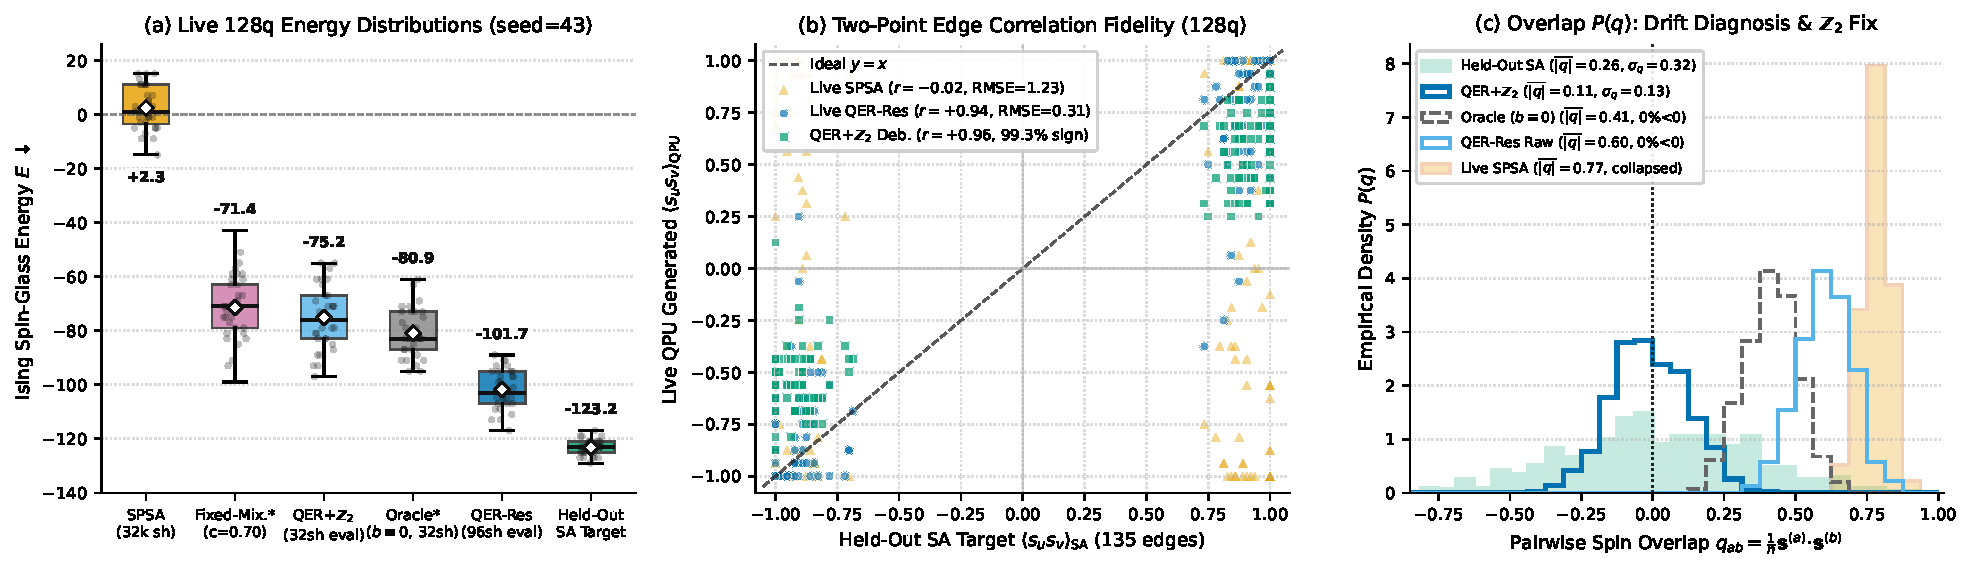
\includegraphics[width=\textwidth]{analysis/fig_live_generative_audit.pdf}
\caption{\textbf{Live $128$-Qubit \texttt{ibm\_kingston} Generative Distribution Audit (\texttt{seed=43}, Raw Extracted Bitstrings).} (a) Energy distributions comparing live $96$-dir \texttt{SPSA}, a single-shot fixed-mixer oracle-sign circuit$^*$ ($c{=}0.70$, unoptimized schedule, $N{=}128$), blind \texttt{QER-Res} + batch-$\mathbb{Z}_2$ debiasing ($32$ eval sh/step), oracle-sign reverse-diffusion template$^*$ ($J{=}{-}0.70J^{\text{sg}}, b{\equiv}0$, $32$ eval sh/step), raw \texttt{QER-Res} ($96$ eval sh/step), and held-out SA targets ($N{=}32$). (b) Two-point edge-correlation scatter $\langle s_u s_v\rangle_{\text{QPU}}$ vs.\ $\langle s_u s_v\rangle_{\text{SA}}$ across all $135$ edges ($N{=}32$): \texttt{QER-Res} ($r{=}+0.945$) and \texttt{QER-Res}+$\mathbb{Z}_2$ debiasing ($r{=}+0.956$, $99.3\%$ sign match) track the diagonal cleanly while live \texttt{SPSA} ($r{=}-0.016$) scatters randomly. (c) Edwards--Anderson pairwise overlap $P(q)$: session-specific hardware offsets shift even the exact $b{\equiv}0$ template ($\overline{|q|}{=}0.41$) and raw \texttt{QER-Res} ($\overline{|q|}{=}0.60$) into one sector ($0\%$ negative pairs), while live \texttt{SPSA} collapses ($\overline{|q|}{=}0.77$); batch-centered $\mathbb{Z}_2$ debiasing centers the distribution ($\overline{|q|}{=}0.11, \sigma_q{=}0.13$, though over-centering below the i.i.d.\ null $|m|{=}0.141$, see text).}
\label{fig:live_gen_audit}
\end{figure}

\begin{table}[t!]
\centering
\caption{\textbf{Matched-$N$ Distribution Audit on Extracted Raw Live $128$--$156$q \texttt{ibm\_kingston} Bitstrings vs.\ Live Oracle Controls and Classical Inverse-Ising References.} All $8$ live runs reconstruct Table~\ref{tab:heron_spinglass}'s energies to exact precision from archived IBM Job IDs (Table~\ref{tab:ibm_job_ledger}). Because $\bar{q} \equiv (N\langle m_i^2\rangle{-}1)/(N{-}1)$ holds identically (verified to $0.0$ error), $\bar{q}$ is redundant given $\langle m_i^2\rangle$ (at $N{=}32$, i.i.d.\ $\mathbb{Z}_2$ null $\overline{|m_i|}{=}0.141$ and forced zero batch mean gives $\bar{q}{=}{-}1/31{=}{-}0.032$); independent distributional evidence comes from overlap width ($\overline{|q|} / \sigma_q$) and two-point edge correlations at matched $N$. $^*$Oracle controls receive ground-truth signs $J^{\text{sg}}$ as input and have unmatched eval shots ($32$ sh/step vs.\ $96$ sh/step for raw \texttt{QER-Res}); classical MM/PL Gibbs and SA references are reported at both $N{=}32$ and $N{=}128$ so sampling noise floors match.}
\label{tab:heron_gen_audit}
\small
\resizebox{\textwidth}{!}{%
\begin{tabular}{@{}lccccccccc@{}}
\toprule
\textbf{Live QPU Run / Reference} & \textbf{Eval Sh / $N$} & \textbf{Mean $E \pm \sigma$ $\downarrow$} & \textbf{Sat \% $\uparrow$} & $\overline{|m_i|}$ & \textbf{Edge RMSE $\downarrow$} & \textbf{Edge $r$ $\uparrow$} & \textbf{Edge Sign $\uparrow$} & \textbf{$\overline{|q|} / \sigma_q$ ($\bar{q}$)} & \textbf{$W_1$ $\downarrow$} \\
\midrule
\multicolumn{10}{l}{\textit{Instance 1: Live $128$q \texttt{ibm\_kingston} (\texttt{seed=42}, $|E|{=}135$; cross-day: \texttt{QER-Res} Nov 18, controls Nov 20)}} \\
\midrule
Untrained QPU ($\theta{=}0$, Live) & $96{\times}4$ / $32$ & $-5.1 \pm 10.6$ & $51.9\%$ & $0.485$ & $0.954$ & $+0.099$ & $50.4\%$ & $0.323 / 0.075$ ($+0.32$) & $118.4$ \\
\texttt{Coord-PSR} (Live, $38.9\text{k}$ tr.) & $96{\times}4$ / $32$ & $+10.4 \pm 8.1$ & $46.1\%$ & $0.870$ & $1.296$ & $-0.103$ & $43.0\%$ & $0.807 / 0.045$ ($+0.81$) & $133.9$ \\
\texttt{QER-Res no-zz} (Live, $38.0\text{k}$ tr.) & $96{\times}4$ / $32$ & $-30.1 \pm 10.7$ & $61.1\%$ & $0.558$ & $0.793$ & $+0.503$ & $68.1\%$ & $0.370 / 0.081$ ($+0.37$) & $93.4$ \\
$96$-Dir \texttt{SPSA} (Live, $39.2\text{k}$ tr.) & $96{\times}4$ / $32$ & $-34.9 \pm 5.7$ & $62.9\%$ & $0.830$ & $0.993$ & $+0.324$ & $63.0\%$ & $0.758 / 0.046$ ($+0.76$) & $88.5$ \\
\textbf{\texttt{QER-Res} Raw (Live, $38.0\text{k}$ tr.)} & $96{\times}4$ / $32$ & $\mathbf{-89.1 \pm 9.2}$ & $\mathbf{83.0\%}$ & $0.625$ & $\mathbf{0.403}$ & $\mathbf{+0.905}$ & $\mathbf{95.6\%}$ & $0.473 / 0.092$ ($+0.47$) & $\mathbf{34.4}$ \\
\textit{Ref: Held-Out SA / Class.\ MM / PL ($N{=}32$)} & -- / $32$ & $-123.3 / -119.1 / -111.6$ & $95.7 / 94.1 / 91.3\%$ & $0.148 / .138 / .149$ & $0.065 / .107 / .155$ & $+.997 / .993 / .989$ & $100\%$ & $0.255 / 0.314$ ($0.00$) & $0.5 / 4.4 / 11.9$ \\
\textit{Ref: Class.\ MM / PL Gibbs ($N{=}128$)} & -- / $128$ & $-118.5 / -108.8$ & $93.9 / 90.3\%$ & $0.062 / 0.076$ & $0.085 / 0.136$ & $+.996 / .995$ & $100\%$ & $0.248 / 0.176$ ($0.00$) & $4.9 / 14.6$ \\
\midrule
\multicolumn{10}{l}{\textit{Instance 2: Live $128$q \texttt{ibm\_kingston} (\texttt{seed=43}, $|E|{=}135$, Same-Session Nov 20) + Live Oracle Controls \& $\mathbb{Z}_2$ Debiasing}} \\
\midrule
$96$-Dir \texttt{SPSA} (Live, $32.3\text{k}$ tr.) & $96{\times}4$ / $32$ & $+2.3 \pm 7.9$ & $49.1\%$ & $0.842$ & $1.231$ & $-0.016$ & $45.9\%$ & $0.772 / 0.047$ ($+0.77$) & $125.5$ \\
\textbf{\texttt{QER-Res} Raw (Live, $31.1\text{k}$ tr.)} & $96{\times}4$ / $32$ & $\mathbf{-101.7 \pm 7.1}$ & $\mathbf{87.7\%}$ & $0.718$ & $\mathbf{0.308}$ & $\mathbf{+0.945}$ & $\mathbf{97.0\%}$ & $0.597 / 0.094$ ($+0.60$) & $\mathbf{21.5}$ \\
\textbf{\texttt{QER-Res} + Batch-$\mathbb{Z}_2$ Deb.\ (Live)} & $32{\times}4$ / $32$ & $-75.2 \pm 11.4$ & $77.8\%$ & $0.093^\dagger$ & $0.397$ & $\mathbf{+0.956}$ & $\mathbf{99.3\%}$ & $0.110 / 0.133$ ($-0.02^\dagger$) & $48.0$ \\
$^*$Oracle Template ($J{=}{-}0.70J^{\text{sg}}, b{\equiv}0$) & $32{\times}4$ / $32$ & $-80.9 \pm 8.7$ & $80.0\%$ & $0.565$ & $0.457$ & $+0.877$ & $94.8\%$ & $0.408 / 0.094$ ($+0.41$) & $42.3$ \\
$^*$Fixed-Mixer 1-Sh ($c{=}0.40/0.70/1.00$, $N{=}32$)$^\ddagger$ & $1{\times}32$ / $32$ & $-47.0 / -71.4 / -79.7$ & $67.4 / 76.5 / 79.5\%$ & $.185 / .186 / .177$ & $.595 / .421 / .360$ & $+.895 / .955 / .967$ & $96.9 / 99.6 / 99.8\%$ & $.08$--$.10 / .10$--$.13$ ($+.02$) & $76.2 / 51.8 / 43.5$ \\
$^*$Fixed-Mixer 1-Sh ($c{=}0.40/0.70/1.00$, $N{=}128$) & $1{\times}128$ / $128$ & $-47.0 / -71.4 / -79.7$ & $67.4 / 76.5 / 79.5\%$ & $.130 / .139 / .130$ & $.578 / .399 / .339$ & $+.962 / .984 / .987$ & $100\%$ & $.08$--$.10 / .10$--$.13$ ($+.02$) & $76.2 / 51.8 / 43.5$ \\
\textit{Ref: Held-Out SA / Class.\ MM / PL ($N{=}32$)} & -- / $32$ & $-123.2 / -118.0 / -111.3$ & $95.6 / 93.7 / 91.2\%$ & $0.169 / .180 / .160$ & $0.067 / .118 / .150$ & $+.997 / .992 / .990$ & $100\%$ & $0.260 / 0.321$ ($+0.01$) & $0.4 / 5.2 / 11.9$ \\
\textit{Ref: Class.\ MM / PL Gibbs ($N{=}128$)} & -- / $128$ & $-118.2 / -109.6$ & $93.8 / 90.6\%$ & $0.057 / 0.070$ & $0.082 / 0.135$ & $+.997 / .994$ & $100\%$ & $0.234 / 0.176$ ($0.00$) & $5.0 / 13.7$ \\
\midrule
\multicolumn{10}{l}{\textit{Full-Chip $156$q \texttt{ibm\_kingston} (\texttt{seed=42}, $|E|{=}176$, Unpruned, 2026-11-20)}} \\
\midrule
\textbf{\texttt{QER-Res} Raw ($156$q Live, $38.0\text{k}$ tr.)} & $96{\times}4$ / $32$ & $\mathbf{-98.5 \pm 9.6}$ & $\mathbf{78.0\%}$ & $0.548$ & $\mathbf{0.457}$ & $\mathbf{+0.869}$ & $\mathbf{94.3\%}$ & $0.377 / 0.094$ ($+0.38$) & $\mathbf{56.9}$ \\
\textit{Ref: Held-Out SA / Class.\ MM / PL ($N{=}32$)} & -- / $32$ & $-156.1 / -149.2 / -143.4$ & $94.4 / 92.4 / 90.7\%$ & $0.099 / .152 / .140$ & $0.071 / .122 / .145$ & $+.997 / .991 / .988$ & $100\%$ & $0.229 / 0.285$ ($-0.02$) & $0.8 / 6.2 / 12.0$ \\
\textit{Ref: Class.\ MM / PL Gibbs ($N{=}128$)} & -- / $128$ & $-150.7 / -141.8$ & $92.8 / 90.3\%$ & $0.084 / 0.072$ & $0.095 / 0.114$ & $+.994 / .995$ & $100\%$ & $0.250 / 0.181$ ($0.00$) & $4.7 / 13.6$ \\
\bottomrule
\multicolumn{10}{l}{\scriptsize $^\dagger$Batch-centering injects a zero-magnetization prior, over-centering $\overline{|m_i|}{=}0.093$ below the $N{=}32$ i.i.d.\ null ($0.141$) and algebraically pulling $\bar{q}{=}{-}0.019$ toward $-1/31{=}{-}0.032$. $^\ddagger$Fixed-mixer $N{=}32$ metrics average across all $4$ disjoint $32$-shot chunks of the $128$-shot draw; satisfaction increases monotonically through $c{=}1.00$ (optimum at $c{>}1.0$).}
\end{tabular}%
}
\end{table}

\begin{enumerate}[leftmargin=1.4em,itemsep=2pt,topsep=2pt]
  \item \textbf{Two-Point Correlation Fidelity \& Candid Hebbian Scope:} On extracted live bitstrings ($N{=}32$), \texttt{QER-Res} cuts two-point edge-correlation RMSE against held-out SA from $0.954$--$1.296$ (untrained/\texttt{SPSA}/\texttt{Coord-PSR}) down to $0.403$ (\texttt{seed=42}, $r{=}+0.905$, $95.6\%$ sign match, $W_1{=}34.4$), $0.308$ (\texttt{seed=43}, $r{=}+0.945$, $97.0\%$ sign match, $W_1{=}21.5$), and $0.457$ ($156$q, $r{=}+0.869$, $94.3\%$ sign match). On saved checkpoints, live \texttt{QER-Res} recovers $135/135$ ($100.0\%$) of the hidden bond signs on $128$q (\texttt{seed=43}) and $167/176$ ($94.9\%$) on $156$q ($|J|/|b|{=}5.0\times$ and $6.1\times$). \emph{Candid scope caveat:} on this sparse Heavy-Hex spin glass, classical Hebbian sign estimation $\operatorname{sign}(-\langle s_u s_v\rangle_{\text{SA}})$ recovers $100.0\%$ of $J^{\text{sg}}$ trivially from the same samples ($\min|\langle s_u s_v\rangle_{\text{SA}}|{=}0.656$ at $128$q, $0.531$ at $156$q), and \texttt{QER-Res}'s learned couplers closely track a uniform signed template ($c_{\text{unif}}{=}0.697$, $\text{CV}{=}10.3\%$, $r(J, c_{\text{unif}}\operatorname{sign}(c_{\text{SA}})){=}+0.995$, closely matching Adam's $9$-step LR sum $\sum_t\text{lr}_t{=}0.845$ minus decay), with only modest residual correlation to $|\langle s_u s_v\rangle_{\text{SA}}|$ ($r{=}+0.266, t{=}+3.2$ at $128$q; $r{=}+0.327, t{=}+4.6$ at $156$q) and endpoint degree ($r{=}-0.207 / -0.211$). Moreover, noiseless classical inverse-Ising references fit on the same SA samples (Bethe moment-matching and Besag pseudolikelihood~\cite{besag1975pl} + Gibbs sampling) reach $90.3\%$--$94.1\%$ satisfaction ($0.107$--$0.155$ RMSE at matched $N{=}32$; $0.082$--$0.136$ at $N{=}128$). We therefore do \emph{not} claim that QPU-in-the-loop training outperforms a $0$-training-shot classical Hebbian estimate ($J{=}c\hat{J}_{\text{Hebbian}}$) plugged into one circuit on a standalone Ising spin glass; rather, the experiment validates \texttt{QER-Res} as an $\mathcal{O}(1)$-circuit hardware trainer where closed-form moment matching is unavailable.
  \item \textbf{Unmatched Live Oracle Controls ($32$ vs.\ $96$ Eval Shots):} On the \texttt{seed=43} $128$q subgraph, we ran two live oracle-sign controls \emph{handed all $135$ true signs $J^{\text{sg}}$}: (i) an unconditioned single-shot fixed-mixer Ising circuit ($J{=}{-}cJ^{\text{sg}}, b{\equiv}0, \mathbf{x}_t{\equiv}\mathbf{0}$, unoptimized fixed mixer schedule, $128$ raw shots) reaching $67.4\%$ ($c{=}0.40$), $76.5\%$ ($c{=}0.70$), and $79.5\%$ ($c{=}1.00$; still rising monotonically, so its peak lies at $c{>}1.0$), with symmetric unbiased draws ($\overline{|m_i|}{=}0.177$--$0.186$ at $N{=}32$, $0.130$--$0.139$ at $N{=}128$; matched-$N{=}32$ RMSE $0.360$, $r{=}+0.967$ at $c{=}1.00$); and (ii) a $4$-step reverse-diffusion uniform oracle template ($J{=}{-}0.70J^{\text{sg}}, b{\equiv}0$, $32$ eval sh/step) scoring $80.0\%$ ($E{=}-80.9$, RMSE $0.457$, $r{=}+0.877$). Crucially, because raw \texttt{QER-Res} ($87.7\%$) used $3\times$ more evaluation shots per step ($96$ vs.\ $32$) and non-zero learned biases ($\overline{|b|}{=}0.139$), the $87.7\%$ vs.\ $80.0\%$ difference is \emph{not} a matched comparison; at matched $32$ eval shots/step (with debiasing), \texttt{QER-Res} scores $77.8\%$, slightly below the $80.0\%$ raw template (though with lower Edge RMSE $0.397$ vs.\ $0.457$ and higher $r{=}+0.956$ vs.\ $+0.877$). A controlled $2{\times}2{\times}2$ factorial over $\{\text{template}, \text{QER-Res}\}\times\{\text{raw}, \text{debias}\}\times\{32, 96\text{ eval sh}\}$ plus an extended $c{>}1$ blind-Hebbian scan is needed in future QPU allocations to separate these effects cleanly.
  \item \textbf{Forensic Proof of Session-Specific Hardware Drift \& Candid Debiasing Caveats:} Auditing $\overline{|m_i|}$ shows that \emph{every} standard deterministic reverse-diffusion run on \texttt{ibm\_kingston} locks into a single $\mathbb{Z}_2$ sector ($0\%$ negative overlaps), including \textbf{Untrained QPU ($\theta{=}0$: $\overline{|m_i|}{=}0.485$)} and the \textbf{exact $b_i{\equiv}0$ Oracle Template ($\overline{|m_i|}{=}0.565$)}, with raw \texttt{QER-Res} at $0.548$--$0.718$ and noisy \texttt{SPSA}/\texttt{Coord-PSR} collapsing severely into high-energy states ($0.830$--$0.870$, $\overline{|q|}{=}0.758$--$0.807$). A noiseless $128$q-equivalent $\theta{=}0$ simulation of identical \texttt{sample\_qerd\_batch} stays unbiased ($\overline{|m_i|}{=}0.146$, $45.0\%{<}0$), whereas live \texttt{ibm\_kingston} $\theta{=}0$ grows monotonically across reverse steps $t{=}4{\to}1$ ($\overline{|m_i|}{=}0.240{\to}0.381{\to}0.437{\to}0.485$). Regressing $m_i(\theta{=}0)$ directly against the $512$-shot depth-$0$ readout calibration yields only weak negative correlation ($r{=}-0.185, R^2{=}3.4\%, t{=}-2.11$ vs.\ \texttt{ro\_offset}; $r{=}+0.089, R^2{=}0.8\%$ vs.\ \texttt{ro\_scale}), ruling out depth-$0$ readout asymmetry as the main driver (the tiny negative residual reflects subtracting finite-shot \texttt{ro\_offset}). Instead, independent \emph{same-day} (2026-11-20) runs exhibit significant per-qubit magnetization correlation ($r{=}+0.318, t{=}+3.8$ between Untrained $\theta{=}0$ and Oracle $b{\equiv}0$; $r{=}+0.281, t{=}+3.3$ between Oracle $b{\equiv}0$ and \texttt{QER-Res} \texttt{seed=43}), whereas \emph{cross-day} (Nov~18 vs.\ Nov~20) correlations vanish ($r{=}+0.052, -0.085$), directly confirming session-specific in-circuit hardware drift amplified by deterministic reverse diffusion. Applying batch-centered $\mathbb{Z}_2$ debiasing ($\tilde{\mathbf{z}}_t = \mathbf{z}_t - \overline{\mathbf{z}}_t$, $0$ extra training shots, $32$ eval sh/step) live on \texttt{seed=43} yields $77.8\%$ satisfied bonds, $r{=}+0.956$, $99.3\%$ ($134/135$) edge-sign accuracy, and overlap width $\overline{|q|}{=}0.110, \sigma_q{=}0.133$ ($\max|q|{=}0.406$); however, batch-centering injects a zero-magnetization prior that slightly over-centers $\overline{|m_i|}{=}0.093$ below the i.i.d.\ null ($0.141$, mechanically pulling $\bar{q}{=}-0.019$ near $-1/31$), and the concurrent eval-shot reduction ($96{\to}32$) prevents attributing the $87.7\%{\to}77.8\%$ energy shift solely to debiasing. A randomized global-$X$ twirl during inference is a cleaner prior-free alternative for future hardware runs.
\end{enumerate}

\subsection{Secondary 128-Qubit Validation: Conditional Human Promoter DNA}
\label{sec:heron_dna}
As a second $128$-qubit hardware benchmark with zero neural autoencoder, we bijectively mapped $64\text{ bp}$ \emph{H.\ sapiens} promoter sequences onto $128$ \texttt{ibm\_kingston} qubits via $2$ qubits/nucleotide ($\text{A}{=}(-1,-1), \text{T}{=}(-1,+1), \text{G}{=}(+1,-1), \text{C}{=}(+1,+1)$, $|E|{=}135$ native edges including $50/64$ intra-base CZ couplers, $L{=}2$, $T{=}3$, $38{,}016$--$39{,}168$ shots, $N{=}32$ draws; Figure~\ref{fig:heron_live}(c), Table~\ref{tab:heron_dna}). Using class-matched biophysical target filtering (allowing naturally AT-rich TATA boxes alongside GC-rich non-TATA promoters) and one-hot class conditioning ($[1,0]$ TATA vs.\ $[0,1]$ non-TATA via $W_{\text{cond}}\in\mathbb{R}^{128\times 2}$), we executed all four live $128$-qubit hardware models within the same \texttt{ibm\_kingston} calibration session (sharing RO job \texttt{dbvoq3thdvas73biero0}): untrained QPU, \texttt{QER-Res}, equal-shot Chain-Rule $96$-direction \texttt{SPSA}, and zero-$ZZ$ \texttt{QER-Res no-zz}.

\begin{table}[t!]
\centering
\caption{\textbf{Same-Session Live $128$-Qubit ($64\text{ bp}$) \texttt{ibm\_kingston} Fixed-TATA Human Promoter DNA Suite ($L{=}2, T{=}3$, $38\text{k}$--$39\text{k}$ Shots, $N{=}32$).} Live \texttt{QER-Res} beats equal-shot Chain-Rule \texttt{SPSA} by $+27.6\text{ pp}$ activity and $+21.9\text{ pp}$ validity while reaching $75.0\%$ TATA conditioning; live \texttt{no-zz} candidly isolates $1$-body positional dominance on DNA at $L{=}2$.}
\label{tab:heron_dna}
\small
\resizebox{\textwidth}{!}{%
\begin{tabular}{@{}lcccccc@{}}
\toprule
\textbf{Model / Live $128$q Control} & \textbf{Oracle Act.\ $\uparrow$} & \textbf{Valid \% $\uparrow$} & \textbf{TATA-Cond $\uparrow$} & \textbf{TSS Inr $\uparrow$} & \textbf{GC \% / $\Delta G^\circ_{37}$} & \textbf{Motif Corr $\uparrow$} \\
\midrule
Untrained $128$q QPU (Live) & $10.6\%$ & $0.0\%$ & $6.2\%$ & $68.8\%$ & $43.5\%$ / $-82.2$ & $-0.249$ \\
Equal-Shot Chain-Rule $96$-Dir \texttt{SPSA} (Live) & $47.5\%$ & $31.2\%$ & $62.5\%$ & $78.1\%$ & $54.4\%$ / $-89.8$ & $+0.299$ \\
\textbf{\texttt{QER-Res} $128$q Live (Ours, $11$ st)} & $\mathbf{75.1\%}$ & $\mathbf{53.1\%}$ & $\mathbf{75.0\%}$ & $\mathbf{81.2\%}$ & $64.1\%$ / $-97.2$ & $+0.547$ \\
\texttt{QER-Res no-zz} ($0$ $ZZ$, Live $128$q Control) & $81.9\%$ & $59.4\%$ & $87.5\%$ & $62.5\%$ & $61.6\%$ / $-95.7$ & $+0.635$ \\
\midrule
\textit{Ref: Classical $1$st-Order Markov} & $73.5\%$ & $53.1\%$ & $37.5\%$ & $90.6\%$ & $59.4\%$ / $-93.4$ & $+0.599$ \\
\textit{Ref: Real Human DNA (Unfiltered / Filtered)} & $75.8\%$ / $100.0\%$ & $34.4\%$ / $87.5\%$ & $56.2\%$ / $31.2\%$ & $65.6\%$ / $75.0\%$ & $58.7\%$ / $74.5\%$ & $+0.657$ / $+0.857$ \\
\bottomrule
\end{tabular}%
}
\end{table}

Evaluated by the independent $1$D-CNN oracle (\texttt{PromoterOracleNet}, $0.933$ held-out ROC-AUC) and SantaLucia~\cite{santalucia1998dna} $\Delta G^\circ_{37}$ thermodynamics, live $128$q \texttt{QER-Res} rises from $10.6\%$ untrained activity ($0.0\%$ valid, $6.2\%$ TATA) to \textbf{$75.1\%$ activity}, \textbf{$53.1\%$ biophysical validity} (matching Classical Markov at $53.1\%$), \textbf{$75.0\%$ TATA-box conditional recovery}, $81.2\%$ TSS initiator match, and $+0.547$ motif correlation—outperforming equal-shot live Chain-Rule $96$-direction \texttt{SPSA} ($47.5\%$ activity, $31.2\%$ valid, $62.5\%$ TATA) by \textbf{$+27.6\text{ pp}$ oracle activity} and \textbf{$+21.9\text{ pp}$ biophysical validity}. However, executing \texttt{QER-Res no-zz} ($0$ two-qubit couplers, retaining $b_i$ and $W_{\text{cond}}$) live on the same $128$-qubit chip yields $81.9\%$ activity and $59.4\%$ validity (removing $135$ noisy CZ gates eliminates $2$Q depolarization, though full $ZZ$ improves TSS initiator $81.2\%$ vs.\ $62.5\%$ and upstream box $96.9\%$ vs.\ $87.5\%$). Thus on conditional DNA at $L{=}2$, single-site positional fields and $W_{\text{cond}}$ already capture most promoter validity (still testing $519$-parameter QPU optimization, where \texttt{QER-Res} beats live \texttt{SPSA} by $+27.6\text{ pp}$), whereas on the $\mathbb{Z}_2$-symmetric frustrated spin glass ($\mathbb{E}[x_i]{=}0$) removing $ZZ$ drops performance by $-21.9\text{ pp}$ ($83.0\%{\to}61.1\%$).

% ==============================================================================
\section{Synthesis of Diagnostic Controls, Related Work, and Conclusion}
\label{sec:discussion}
% ==============================================================================

\subsection{Diagnostic Scorecard: Positive Findings vs.\ Negative Controls}
Because NISQ machine-learning benchmarks are prone to subtle classical shortcuts and hardware artifacts, Table~\ref{tab:scorecard} consolidates our positive experimental findings alongside the specific negative controls that bound each claim (including our $5$-seed whitened-AE vision co-adaptation study, where \texttt{BatchNorm1d} whitening allows classical \texttt{wcond-only} with $\boldsymbol{\theta}{=}\mathbf{0}$ to match full QER accuracy at $100.0\%$ MNIST / $71.5\%$ Fashion, and where $\sim 200$-parameter denoisers exhibit $\text{Rec}\approx 0.000$ prototype collapse until capacity scales to $P\ge 38\text{k}$).

\begin{table}[t!]
\centering
\caption{\textbf{Diagnostic Scorecard of Positive Findings and Bounding Negative Controls Across All Benchmarks.}}
\label{tab:scorecard}
\small
\resizebox{\textwidth}{!}{%
\begin{tabular}{@{}llll@{}}
\toprule
\textbf{Question / Domain} & \textbf{Verified Positive Finding} & \textbf{Bounding Negative Control / Caveat} & \textbf{Implication} \\
\midrule
Non-Equilibrium Reciprocity (\S\ref{sec:mech}) & Off-diag $\cos_h{=}+0.942$--$+0.993$ ($L{=}4$); $3$-ckt \texttt{QER-Res} fixes $2$-ckt MSE sign flip ($-0.288{\to}+0.519$). & Exact $L{=}1$ JVP$\neq$VJP (Prop.~\ref{prop:centered_bias}); Step-$8$ cubic inversion ($-0.185$) and Step-$25$ $\beta{\to}0$ breakdown ($-0.379$). & Validated finite-$\beta$ surrogate, not exact backprop. \\
Shot SNR \& $2$Q Noise (\S\ref{sec:new_controls}) & $+0.882{\to}+0.841$ $4\text{k}$-shot SNR ($>4\times$ SPSA/Coord-PSR); $12$q Heavy-Hex $85.2\%$ vs.\ $86.7\%$ \texttt{Exact-AD}, flat to $p_{2\text{q}}{=}1.5\%$. & All-to-all $528$-CNOT circuits collapse $83.9\%{\to}8.9\%$ at $p_{2\text{q}}{=}1.5\%$; $64$-dir SPSA underperforms $16$-dir at low $P{=}23$. & Scalable NISQ training requires native $0$-SWAP graphs. \\
Zero-Shortcut $12$--$14$q $ZZ$ (\S\ref{sec:hybrid_sim}) & $12$q Stride-$3$ ($L{=}4$): $100\%$ mode cov, $74.8\% / 80.2\%$ acc vs.\ $1.4\%$ \texttt{no-zz}; $13$--$14$q label-q: $99.3\% / 71.0\%$ vs.\ chance. & On $13$q $\{0,1\}$, $10$-way accuracy drops to $2.9\%$ under uncalibrated $L{=}3$ attenuation; float64 \texttt{ClassicalIsing-EP} hits $100\%$. & Confirms genuine $ZZ$ learning; readout calibration needed. \\
Hybrid \texttt{QERLayer} (\S\ref{sec:hybrid_sim}) & Beats unadapted Clean/Noise-Aware \texttt{Exact-AD} ($0.0882$ vs.\ $0.1006$ MSE; $+7.0$--$9.4\text{ pp}$ MNIST hybrid accuracy). & $0$-bwd-shot \texttt{STE} is within $\sim 0.5\sigma$ ($0.0917$) at $1/3\times$ shots when $\boldsymbol{\theta}$ is frozen; $6$-sh Binomial noise matches diversity. & Use \texttt{STE} if $\boldsymbol{\theta}$ frozen; \texttt{QERLayer} when training $\boldsymbol{\theta}$. \\
Live $128$--$156$q Spin Glass (\S\ref{sec:heron_spinglass}--\ref{sec:heron_audit}) & Raw \texttt{QER-Res} reaches $83.0\% / 87.7\%$ ($128$q) and $78.0\%$ ($156$q), $r{=}+0.905$--$+0.945$ edge corr, $100\% / 94.9\%$ sign rec. & Session-specific hardware drift locks $\theta{=}0$ ($\overline{|m_i|}{=}0.485, r{=}+0.318$); learned $J$ tracks uniform Hebbian ($r{=}+0.995$); classical Gibbs $90$--$94\%$. & Batch-$\mathbb{Z}_2$ debiasing restores $\overline{|m_i|}{=}0.093, r{=}+0.956$ ($77.8\%$ sat at $32$ sh). \\
Live $128$q DNA \& Vision (\S\ref{sec:heron_dna}) & DNA \texttt{QER-Res} beats live SPSA ($75.1\%$ vs.\ $47.5\%$ act, $75\%$ TATA); whitened MNIST QER hits $100.0\%$ ($80\text{k}$ sh). & Live DNA \texttt{no-zz} scores $81.9\% / 59.4\%$; whitened-AE \texttt{wcond-only} ($\boldsymbol{\theta}{=}\mathbf{0}$) hits $100.0\%$ MNIST / $71.5\%$ Fashion ($\text{Rec}{=}0$). & $1$-body / $W_{\text{cond}}$ shortcuts dominate $L{=}2$ DNA \& whitened AEs. \\
\bottomrule
\end{tabular}%
}
\end{table}

\subsection{Related Work, Limitations, and Conclusion}
\label{sec:conclusion}
\paragraph{Related Work.}
Coordinate-wise analytic PSR~\cite{mitarai2018psr,schuld2019psr} and adaptive shot-allocation methods (\texttt{iCANS}~\cite{kubler2020icans}, \texttt{Rosalin}~\cite{arrasmith2020rosalin}, doubly stochastic $1$-shot PSR~\cite{sweke2020sgd}) scale linearly in parameter count $P$ per effective sweep. Abbas et~al.~\cite{abbas2023qbp} proved that generic exact quantum backpropagation cannot achieve classical $\mathcal{O}(1)$ query overhead without coherent multi-copy access; \texttt{QER} stays outside this impossibility theorem strictly by restricting to commuting diagonal Ising operators (where simultaneous computational-basis readout replaces tomography or classical shadows~\cite{huang2020shadows}) and accepting a biased local-response surrogate. Constant-query zeroth-order and directional-gradient estimators (SPSA~\cite{spall1992spsa,kandala2017vqe}, QN-SPSA~\cite{gacon2021qnspsa}, MeZO~\cite{malladi2023mezo}, and adaptive forward gradients for PQCs~\cite{coyle2026forward}) preserve generality across arbitrary ansatzes but incur $\mathcal{O}(P)$ directional variance, while Quantum Natural Gradient~\cite{stokes2020qng} incurs metric-estimation overhead. Most closely related to our contrastive mechanism are classical Equilibrium Propagation~\cite{scellier2017ep,laydevant2024ep,scellier2024ep}, Hamiltonian echo backpropagation~\cite{lopezpastor2023echo}, thermal Quantum Boltzmann Machines~\cite{amin2018qbm}, and recent Quantum Equilibrium Propagation formulations using Onsager reciprocity~\cite{wanjura2025qep} or ground-state energy functionals~\cite{scellier2026qep}. Whereas Wanjura \& Marquardt~\cite{wanjura2025qep} and Scellier~\cite{scellier2026qep} exploit stationary or ground-state quantum equilibrium where exact Onsager reciprocity holds, \texttt{QER} operates on \emph{non-stationary, finite-depth Trotter circuits}~\cite{farhi2014qaoa}—where we prove exact reciprocity breaks down (Proposition~\ref{prop:centered_bias}) and characterize the resulting finite-$\beta$ surrogate regime empirically up to $156$ physical qubits. For inverse-Ising distribution learning, classical Boltzmann Contrastive Divergence~\cite{hinton2002cd} and pseudolikelihood estimation~\cite{besag1975pl} provide strong classical baselines (reported in Table~\ref{tab:heron_gen_audit}); \texttt{QER} targets shallow NISQ circuit training~\cite{zhang2024quddpm,cacioppo2023qdiff,parigi2024qdiff,huang2021qgan,rudolph2022ionqgan} where barren plateaus stay mild~\cite{mcclean2018bp,cerezo2021bp,larocca2024bp}.

\paragraph{Limitations.}
Three strict boundaries qualify our conclusions:
\begin{enumerate}[leftmargin=1.4em,itemsep=2pt,topsep=2pt]
  \item \emph{Replication, Baseline Tuning, Session Split, \& Hebbian Scope:} Our live \texttt{ibm\_kingston} ($128$--$156$q) spin-glass benchmarks validate $\mathcal{O}(1)$-circuit QPU-in-the-loop optimization rather than claiming quantum advantage over classical SA, classical inverse-Ising Gibbs solvers ($90.3\%$--$94.1\%$), or a $0$-training-shot classical Hebbian estimate ($J{=}c\hat{J}_{\text{Hebbian}}$) executed on a single circuit (which remains to be benchmarked at matched eval shots alongside an extended $c{>}1$ fixed-mixer scan and non-Hebbian hidden-unit parity benchmarks). Hardware replication spans two $128$q instances (\texttt{seed=42}, used during development with a cross-day 2026-11-18 vs.\ 2026-11-20 session split, and strictly same-session out-of-development \texttt{seed=43}) plus one $156$q run at $N{=}32$ draws per model; multi-run replicates on a single instance are needed for statistical confidence intervals. Similarly, live $128$q \texttt{SPSA} ($96$ dirs $\times 12$ sh) and \texttt{Coord-PSR} ($128$ coords $\times 8$ sh) degraded below initialization under default Adam scaling, warranting dedicated hardware tuning sweeps and a $b_i{\equiv}0$-clamped \texttt{no-zz} control. Comparing $156$q ($78.0\%$) against $128$q ($83.0\%$) is observational across different graph sizes and $P$ ($332$ vs.\ $263$).
  \item \emph{Architectural, Reciprocity, \& Hardware-Drift Boundaries:} The $\mathcal{O}(1)$ estimator holds strictly for commuting diagonal $Z_i, Z_u Z_v$ weights with fixed $R_X$ mixers and lacks a non-asymptotic convergence proof outside the perturbative regime. Exact $\beta{\to}0$ reciprocity breaks down on $ZZ$ couplers at large weights ($-0.379$ Clean at Step~$25$), and even finite $\beta{=}0.45$ briefly turns negative at Step~$8$ ($-0.254 / -0.185$) due to cubic phase curvature, so \texttt{QER-Grad}/\texttt{QERLayer} are biased finite-$\beta$ surrogates rather than exact backpropagation. Moreover, standard deterministic reverse diffusion on \texttt{ibm\_kingston} suffers session-specific single-sector $\mathbb{Z}_2$ locking ($\overline{|m_i|}{=}0.485$--$0.718$, $0\%$ negative overlaps even at $\theta{=}0$ and on an exact $b{\equiv}0$ template); our live batch-centered $\mathbb{Z}_2$ debiasing ($77.8\%$ sat.\ bonds at $32$ eval sh/step, $r{=}+0.956$) injects a zero-magnetization prior that slightly over-centers $\overline{|m_i|}{=}0.093$ below the $0.141$ null and confounds the $96{\to}32$ eval-shot reduction, motivating a prior-free randomized global-$X$ twirl and $2{\times}2{\times}2$ matched-shot factorial in future hardware runs.
  \item \emph{DNA, Vision, \& Hybrid Caveats:} Live $128$q DNA \texttt{no-zz} ($81.9\%$ / $59.4\%$) proves $1$-body positional fields and $W_{\text{cond}}$ drive most DNA validity at $L{=}2$; whitened-AE vision benchmarks allow trivial classical $W_{\text{cond}}$ shortcuts and suffer $\text{Rec}\approx 0$ at $P{\approx}200$; $13$q zero-$W_{\text{cond}}$ achieves $99.3\%$ $2$-way but only $2.9\%$ $10$-way accuracy due to uncalibrated attenuation; hybrid Recall gains are matched by classical $6$-shot Binomial noise; and on $8$q hybrid controls, $0$-backward-shot \texttt{STE} ($0.0917\pm 0.0082$ MSE at $1/3\times$ shots) trails \texttt{QERLayer} ($0.0865$--$0.0882$) by only $\sim 0.5\sigma$ when $\boldsymbol{\theta}$ is frozen.
\end{enumerate}

\paragraph{Conclusion.}
Restricting trainable quantum weights to commuting diagonal Ising operators interleaved with fixed $R_X$ mixers enables simultaneous contrastive probing of all fields and couplers from $2$--$3$ circuit evaluations per sample ($175\times$--$221\times$ fewer circuits/sample than $2P$ PSR for $3$-circuit \texttt{QER-Res}, $263\times$--$332\times$ for $2$-circuit \texttt{QER-Grad}). While exact JVP--VJP reciprocity fails in finite-depth unitary circuits even as $\beta{\to}0$ (Proposition~\ref{prop:centered_bias}) and undergoes transient cubic inversions at large weights, pairing $3$-circuit residual nudging (\texttt{QER-Res}) with $\beta_2$-preconditioned \texttt{StabilizedAdam} and native Heavy-Hex routing delivers $>4\times$ higher $4\text{k}$-shot gradient SNR than $100$-direction SPSA and coordinate PSR across $6$--$14$ qubits, tracks within $1.5\text{ pp}$ of noiseless \texttt{Exact-AD} on $12$-qubit Heavy-Hex spin glasses up to $p_{2\text{q}}{=}1.5\%$ CNOT error, and recovers frustrated two-point spin-glass correlations on live $128$--$156$-qubit \texttt{ibm\_kingston} hardware ($83.0\%$ and $87.7\%$ raw sector-locked satisfied bonds with $r{=}+0.905$--$+0.945$ edge correlation, $77.8\%$ batch-debiased with $r{=}+0.956$ and $99.3\%$ edge-sign match at $32$ eval sh/step, and $78.0\%$ across all $156$ physical qubits). Code, raw bitstring audits, and the archived IBM Quantum Runtime Job ID ledger will be released publicly upon publication.

\paragraph{AI Assistance Disclosure.}
Large Language Model (LLM) assistants were used during this project to draft and copyedit English prose, format LaTeX tables and figures, and assist with code modularization, Qiskit Runtime batching implementation, and unit-test scaffolding. The human author directed the research questions, hardware and simulator experiments, and negative controls, cross-checked reported metrics against saved experimental outputs, verified library behavior via automated tests, and reviewed every derivation, citation, and stated limitation. No unverified experimental numbers or references are included, and the author takes full responsibility for the entire manuscript.

% ==============================================================================
% Bibliography
% ==============================================================================
\begin{thebibliography}{99}
\small
\setlength{\itemsep}{2pt}
\bibitem{abbas2023qbp} A.~Abbas, R.~King, H.-Y. Huang, W.~J. Huggins, R.~Movassagh, D.~Gilboa, and J.~R. McClean. On quantum backpropagation, information reuse, and cheating measurement collapse. {\em NeurIPS}, 2023.
\bibitem{amin2018qbm} M.~H. Amin, E.~Andriyash, J.~Rolfe, B.~Kulchytskyy, and R.~Melko. Quantum Boltzmann machine. {\em Physical Review X}, 8(2):021050, 2018.
\bibitem{arrasmith2020rosalin} A.~Arrasmith, L.~Cincio, R.~D. Somma, and P.~J. Coles. Operator sampling for shot-frugal optimization in variational algorithms. {\em arXiv:2004.06252}, 2020.
\bibitem{besag1975pl} J.~Besag. Statistical analysis of non-lattice data. {\em Journal of the Royal Statistical Society: Series D (The Statistician)}, 24(3):179--195, 1975.
\bibitem{cacioppo2023qdiff} A.~Cacioppo, L.~Colantonio, S.~Bordoni, and S.~Giagu. Quantum diffusion models. {\em arXiv:2311.15444}, 2023.
\bibitem{cerezo2021bp} M.~Cerezo, A.~Sone, T.~Volkoff, L.~Cincio, and P.~J. Coles. Cost function dependent barren plateaus in shallow parametrized quantum circuits. {\em Nature Communications}, 12:1791, 2021.
\bibitem{coyle2026forward} B.~Coyle, S.~Raj, V.~Umathe, E.~A. Cherrat, and E.~Kashefi. Adaptive directional gradients for parameterised quantum circuits. {\em arXiv:2606.09734}, 2026.
\bibitem{farhi2014qaoa} E.~Farhi, J.~Goldstone, and S.~Gutmann. A quantum approximate optimization algorithm. {\em arXiv:1411.4028}, 2014.
\bibitem{gacon2021qnspsa} J.~Gacon, C.~Zoufal, G.~Carleo, and S.~Woerner. Simultaneous perturbation stochastic approximation of the quantum Fisher information. {\em Quantum}, 5:567, 2021.
\bibitem{heusel2017fid} M.~Heusel et~al. GANs trained by a two time-scale update rule converge to a local Nash equilibrium. {\em NeurIPS}, 2017.
\bibitem{hinton2002cd} G.~E. Hinton. Training products of experts by minimizing contrastive divergence. {\em Neural Computation}, 14(8):1771--1800, 2002.
\bibitem{ho2020ddpm} J.~Ho, A.~Jain, and P.~Abbeel. Denoising diffusion probabilistic models. {\em NeurIPS}, 2020.
\bibitem{huang2020shadows} H.-Y. Huang, R.~Kueng, and J.~Preskill. Predicting many properties of a quantum system from very few measurements. {\em Nature Physics}, 16:1050--1057, 2020.
\bibitem{huang2021qgan} H.-L. Huang et~al. Experimental quantum generative adversarial networks for image generation. {\em Physical Review Applied}, 16(2):024051, 2021.
\bibitem{kandala2017vqe} A.~Kandala et~al. Hardware-efficient variational quantum eigensolver for small molecules and quantum magnets. {\em Nature}, 549:242--246, 2017.
\bibitem{kingma2015adam} D.~P. Kingma and J.~Ba. Adam: A method for stochastic optimization. {\em ICLR}, 2015.
\bibitem{kubler2020icans} J.~M. K{\"u}bler, A.~Arrasmith, L.~Cincio, and P.~J. Coles. An adaptive optimizer for measurement-frugal variational algorithms. {\em Quantum}, 4:263, 2020.
\bibitem{larocca2024bp} M.~Larocca et~al. A review of barren plateaus in variational quantum computing. {\em arXiv:2405.00781}, 2024.
\bibitem{laydevant2024ep} J.~Laydevant, D.~Markovic, and J.~Grollier. Training an Ising machine with equilibrium propagation. {\em Nature Communications}, 15:3671, 2024.
\bibitem{lopezpastor2023echo} V.~L{\'o}pez-Pastor and F.~Marquardt. Self-learning machines based on Hamiltonian echo backpropagation. {\em Physical Review X}, 13(3):031020, 2023.
\bibitem{malladi2023mezo} S.~Malladi et~al. Fine-tuning language models with just forward passes. {\em NeurIPS}, 2023.
\bibitem{mcclean2018bp} J.~R. McClean et~al. Barren plateaus in quantum neural network training landscapes. {\em Nature Communications}, 9:4812, 2018.
\bibitem{mitarai2018psr} K.~Mitarai, M.~Negoro, M.~Kitagawa, and K.~Fujii. Quantum circuit learning. {\em Physical Review A}, 98(3):032309, 2018.
\bibitem{naeem2020prdc} M.~F. Naeem, S.~J. Oh, Y.~Uh, Y.~Choi, and J.~Yoo. Reliable fidelity and diversity metrics for generative models. {\em ICML}, 2020.
\bibitem{parigi2024qdiff} M.~Parigi, S.~Martina, and F.~Caruso. Quantum-noise-driven generative diffusion models. {\em Advanced Quantum Technologies}, 2024.
\bibitem{rudolph2022ionqgan} M.~S. Rudolph et~al. Generation of high-resolution handwritten digits with an ion-trap quantum computer. {\em Physical Review X}, 12(3):031010, 2022.
\bibitem{santalucia1998dna} J.~SantaLucia Jr. A unified view of polymer, dumbbell, and oligonucleotide DNA nearest-neighbor thermodynamics. {\em Proc.\ Natl.\ Acad.\ Sci.}, 95(4):1460--1465, 1998.
\bibitem{scellier2017ep} B.~Scellier and Y.~Bengio. Equilibrium propagation: Bridging the gap between energy-based models and backpropagation. {\em Frontiers Comput.\ Neurosci.}, 11:24, 2017.
\bibitem{scellier2024ep} B.~Scellier, M.~Ernoult, J.~Kendall, and S.~Kumar. Energy-based learning algorithms for analog computing: A comparative study. {\em NeurIPS}, 2023.
\bibitem{scellier2026qep} B.~Scellier. Quantum equilibrium propagation: Gradient-descent training of quantum systems. {\em APL Quantum}, 3(2):026117, 2026.
\bibitem{schuld2019psr} M.~Schuld, V.~Bergholm, C.~Gogolin, J.~Izaac, and N.~Killoran. Evaluating analytic gradients on quantum hardware. {\em Physical Review A}, 99(3):032331, 2019.
\bibitem{sohldickstein2015} J.~Sohl-Dickstein, E.~Weiss, N.~Maheswaranathan, and S.~Ganguli. Deep unsupervised learning using nonequilibrium thermodynamics. {\em ICML}, 2015.
\bibitem{spall1992spsa} J.~C. Spall. Multivariate stochastic approximation using a simultaneous perturbation gradient approximation. {\em IEEE Trans.\ Autom.\ Control}, 37(3):332--341, 1992.
\bibitem{stokes2020qng} J.~Stokes, J.~Izaac, N.~Killoran, and G.~Carleo. Quantum natural gradient. {\em Quantum}, 4:269, 2020.
\bibitem{sweke2020sgd} R.~Sweke, F.~Wilde, J.~Meyer, M.~Schuld, P.~K. F{\"a}hrmann, B.~Meynard-Piganeau, and J.~Eisert. Stochastic gradient descent for hybrid quantum-classical optimization. {\em Quantum}, 4:314, 2020.
\bibitem{wanjura2025qep} C.~C. Wanjura and F.~Marquardt. Quantum equilibrium propagation for efficient training of quantum systems based on Onsager reciprocity. {\em Nature Communications}, 16:6595, 2025.
\bibitem{zhang2024quddpm} B.~Zhang, P.~Xu, X.~Chen, and Q.~Zhuang. Generative quantum machine learning via denoising diffusion probabilistic models. {\em Physical Review Letters}, 132(10):100602, 2024.
\end{thebibliography}

% ==============================================================================
% APPENDICES
% ==============================================================================
\clearpage
\appendix

\section{Analytical Derivations (Propositions~\ref{prop:centered_bias}--\ref{prop:vjp})}
\label{app:proofs}

\subsection{Proof of Proposition~\ref{prop:centered_bias} (Centered Bias, Exact \texorpdfstring{$L{=}1$}{L=1} Formula, and Kubo Regime)}
\paragraph{1. Centered $\mathcal{O}(\beta^2)$ Cancellation.}
Write $O_k(\mathbf{h}) = \operatorname{Tr}[\mathcal{O}_k\,\mathcal{M}_L\circ\cdots\circ\mathcal{M}_1(\rho_0)]$ as a smooth bounded observable of visible fields $\mathbf{h}_{\text{vis}} = \mathbf{h}_{\text{free}} + \Delta\mathbf{h}$. Expanding to third order at $\Delta\mathbf{h}=\pm\beta\mathbf{y}$ ($\|\mathbf{y}\|_\infty \le 1$):
\begin{equation}
  O_k(\mathbf{h}_{\text{free}}\pm\beta\mathbf{y}) = O_k(\mathbf{h}_{\text{free}}) \pm \beta\langle\nabla_{\mathbf{h}} O_k, \mathbf{y}\rangle + \frac{\beta^2}{2}\mathbf{y}^\top(\nabla_{\mathbf{h}}^2 O_k)\mathbf{y} \pm \frac{\beta^3}{6} D_{\mathbf{y}}^3 O_k + \mathcal{O}(\beta^4).
\end{equation}
Taking $(O_k(\mathbf{h}_{\text{free}}{+}\beta\mathbf{y}) - O_k(\mathbf{h}_{\text{free}}{-}\beta\mathbf{y}))/(2\beta)$ cancels $O_k(\mathbf{h}_{\text{free}})$ and all even-order terms identically for any $L\ge 1$ and depolarizing channel, leaving $\langle\nabla_{\mathbf{h}} O_k, \mathbf{y}\rangle + \mathcal{O}(\beta^2)$ in $2$ circuits per sample because all $\mathcal{O}_k\in\{Z_i, Z_u Z_v\}$ commute in the computational basis.

\paragraph{2. Exact $L{=}1$ Two-Qubit Analytical Calculation.}
For $n{=}2, L{=}1$, $|\psi_1\rangle = U_X U_Z |++\rangle$ with $U_Z = \exp[-i\frac{g}{2}(h_1 Z_1 + h_2 Z_2 + J Z_1 Z_2)]$ and $U_X = \exp[-i\frac{\phi}{2}(X_1+X_2)]$. In the Heisenberg picture, $U_X^\dagger Z_m U_X = \cos\phi\, Z_m + \sin\phi\, Y_m$ and $U_Z^\dagger Y_1 U_Z = \cos(g(h_1+J Z_2)) Y_1 + \sin(g(h_1+J Z_2)) X_1$. Since $\langle +|Z|+\rangle=\langle +|Y|+\rangle=0$ and $\langle +|X|+\rangle=1$, averaging over the two eigenvalues $Z_2\in\{\pm 1\}$ gives
\begin{equation}
  \langle Z_1 \rangle = \sin\phi\cdot\frac{1}{2}\big[\sin(g(h_1+J)) + \sin(g(h_1-J))\big] = \sin\phi\sin(gh_1)\cos(gJ).
\end{equation}
Differentiating yields $\partial\langle Z_1\rangle/\partial J = -g\sin\phi\sin(gh_1)\sin(gJ)$ and $\partial\langle Z_1\rangle/\partial h_2 \equiv 0$. For $Z_1 Z_2$, expanding $U_X^\dagger Z_1 Z_2 U_X = (\cos\phi Z_1 + \sin\phi Y_1)(\cos\phi Z_2 + \sin\phi Y_2)$ and noting $[Z_1 Z_2, Y_1 Y_2]=0$ yields:
\begin{equation}
  \langle Z_1 Z_2\rangle = \sin\phi\cos\phi\sin(gJ)\big[\cos(gh_1)+\cos(gh_2)\big] + \sin^2\phi\sin(gh_1)\sin(gh_2).
\end{equation}
Differentiating with respect to $h_1$ yields Eq.~\eqref{eq:l1_jvp} directly, which we verify numerically to $10^{-10}$ in \nolinkurl{tests/test_qerd.py}. Hence $\partial\langle Z_1 Z_2\rangle/\partial h_1 \neq \partial\langle Z_1\rangle/\partial J$ even as $\beta\to 0$.

\paragraph{3. Qualitative Quasi-Stationary Kubo/Onsager Reciprocity.}
Consider continuous evolution $U(T)=e^{-iTH(\boldsymbol{\lambda})}$ with real-symmetric $H(\boldsymbol{\lambda}) = H_X + \sum_a \lambda_a O_a$ and real initial state $|\psi_0\rangle=|+\rangle^{\otimes n}$. By Duhamel's formula,
\begin{equation}
  \frac{\partial\langle O_a(T)\rangle}{\partial\lambda_b} = \int_0^T \langle\psi_0|\,i[O_b(s), O_a(T)]\,|\psi_0\rangle\,ds,
\end{equation}
where $O(t)=e^{itH}Oe^{-itH}$. Applying complex conjugation $K$ in the $Z$-basis ($K|\psi_0\rangle=|\psi_0\rangle$, $K O_a K=O_a$, $K e^{itH} K = e^{-itH}$) gives $\langle\psi_0|i[O_b(s), O_a(T)]|\psi_0\rangle = \langle\psi_0|i[O_a(-T), O_b(-s)]|\psi_0\rangle$. Whenever $|\psi_0\rangle$ is stationary under $H$ ($[H,|\psi_0\rangle\langle\psi_0|]=0$), time-translation invariance—shifting first by $+T$ and then by $+s$—gives
\begin{equation}
  \langle\psi_0|\,i[O_a(-T), O_b(-s)]\,|\psi_0\rangle = \langle\psi_0|\,i[O_a(0), O_b(T-s)]\,|\psi_0\rangle = \langle\psi_0|\,i[O_a(s), O_b(T)]\,|\psi_0\rangle,
\end{equation}
and integrating over $s\in[0,T]$ yields exact reciprocity $\partial\langle O_a(T)\rangle/\partial\lambda_b = \partial\langle O_b(T)\rangle/\partial\lambda_a$. Because $|+\rangle^{\otimes n}$ is an eigenstate of $H_X$, this motivates strong reciprocity when diagonal perturbations are weak relative to $H_X$ (small $|\boldsymbol{\theta}|$), and explains why reciprocity degrades as $|\boldsymbol{\theta}|$ grows away from stationarity. Importantly, in our operational circuit $[H, |\psi_0\rangle\langle\psi_0|]\neq 0$ even at $\boldsymbol{\theta}{=}\mathbf{0}$ due to nonzero data-pinning fields $\lambda(\tau)\mathbf{x}_t\in[0.28,0.80]$, and evolution uses discrete Trotter steps with mixer angles $\approx 1$--$2\text{ rad}$ rather than continuous time; thus this argument provides qualitative regime intuition rather than a discrete-circuit convergence guarantee. \qed

\subsection{Proof of Proposition~\ref{prop:dilution} (Regression-Dilution Analysis)}
Under $\mathbf{x}_0 = \boldsymbol{\mu}_t(\mathbf{x}_t)+\boldsymbol{\delta}_t$ ($\mathbb{E}[\boldsymbol{\mu}_t\odot\boldsymbol{\delta}_t]=\mathbf{0}$) and $\mathbf{z}_{\text{mid}}=\gamma\boldsymbol{\mu}_t+\boldsymbol{\eta}_s$, forward OLS ($\mathbf{z}_{\text{mid}}\sim g\mathbf{x}_0$) converges as $w_0{\to}0$ to
\begin{equation}
  g_t^{\text{fwd},*} = \frac{\mathbb{E}[(\gamma\boldsymbol{\mu}_t+\boldsymbol{\eta}_s)\odot(\boldsymbol{\mu}_t+\boldsymbol{\delta}_t)]}{\mathbb{E}[\mathbf{x}_0^2]} = \gamma\,\frac{\mathbb{E}[\boldsymbol{\mu}_t^2]}{\mathbb{E}[\boldsymbol{\mu}_t^2]+\mathbb{E}[\boldsymbol{\delta}_t^2]} = \gamma R_t^2 < \gamma.
\end{equation}
At heavy noise ($R_T^2\ll 1$), dividing $\mathbf{z}_{\text{raw}}$ by $g_t^{\text{fwd},*}$ amplifies predictions by $R_t^{-2}\gg 1$ toward $\{\pm 1\}^D$ corners. Conversely, inverse OLS ($\mathbf{x}_0 \sim a_t\mathbf{z}_{\text{mid}}$) minimizes $\mathbb{E}[(a_t\mathbf{z}_{\text{mid}}-\mathbf{x}_0)^2]$ directly, giving $a_t^* = \gamma\mathbb{E}[\boldsymbol{\mu}_t^2]/(\gamma^2\mathbb{E}[\boldsymbol{\mu}_t^2]+\sigma_s^2)\xrightarrow{\sigma_s^2\to 0}\gamma^{-1}$ ($0.00\%$ boundary clipping on $[0.2,2.0]$ vs.\ $7.42\%$ for forward OLS). \qed

\subsection{Scale-Invariant Surrogate VJP Scope (Proposition~\ref{prop:vjp})}
Normalizing $\tilde{\mathbf{u}}_m = \mathbf{g}_{\text{out},m}/s_m$ with $s_m = \|\mathbf{g}_{\text{out},m}\|_\infty + 10^{-8}$ ensures $|\beta\tilde{\mathbf{u}}_m| \le \beta$ stays inside the linear $R_Z$ response band regardless of upstream loss magnitude, while multiplying by $s_m$ restores gradient scale. Rather than assuming exact unitary reciprocity, Eq.~\eqref{eq:qerlayer} relies on our empirically verified off-diagonal visible-field alignment ($\cos_h^{\text{off}} \in [+0.942, +0.993]$ at $L{=}4$, Table~\ref{tab:exact_recip}) and early/mid-training $ZZ$ alignment. When $\boldsymbol{\theta}$ is frozen, \texttt{QERLayer(backward\_mode="ste")} provides a $0$-backward-shot control directly passing $\mathbf{g}_{\text{out},m}/g$ through the layer. \qed

% ==============================================================================
\section{Experimental Specifications and Live IBM Job ID Reproducibility Ledger}
\label{app:specs}
To ensure full reproducibility without external macro dependencies, we document every benchmark protocol and archive all live \texttt{ibm\_kingston} Job IDs below:
\begin{itemize}[leftmargin=1.4em,itemsep=2pt]
  \item \textbf{Native Heavy-Hex Frustrated Spin Glass (\S\ref{sec:new_controls} \& \S\ref{sec:heron_spinglass}):} Given a connected $n$-qubit subgraph $G=(V,E)$ selected greedily from \texttt{ibm\_kingston} minimizing readout ($3r_v + 0.2\mathbf{1}_{r_v>0.045}$) and CZ ($1.5e_{uv}+0.1\mathbf{1}_{e_{uv}>0.015}$) error penalties ($128$q: $|E|{=}135$; $156$q full chip: $|E|{=}176$; $12$q: $|E|{=}11$), random bonds $J^{\text{sg}}_{uv}\in\{-1,+1\}$ are drawn i.i.d.\ with seed $42$ or $43$. Target configurations are sampled via vectorized Simulated Annealing ($128$ chains, $120$ sweeps at $128$--$156$q; $64$ chains, $80$ sweeps at $12$q) and $\mathbb{Z}_2$-augmented ($\{\mathbf{s}_m,-\mathbf{s}_m\}$) so $\mathbb{E}[x_i]{=}0$.
  \item \textbf{$12$-Qubit Stride-$3$ Correlated Cluster (\S\ref{sec:hybrid_sim}):} Eight discrete modes $\mathbf{x}_m\in\{\pm 1\}^{12}$ defined by $x_m[q] = s_{q\bmod 3}$ for $(s_0,s_1,s_2)\in\{\pm 1\}^3$ (three disjoint $4$-qubit ferromagnetic cliques $\{0,3,6,9\}, \{1,4,7,10\}, \{2,5,8,11\}$; $\mathbb{E}[x_i]{=}0$, intra-cluster correlation $+1$, inter-cluster $0$, $40\text{k}$ total shots).
  \item \textbf{Zero-$W_{\text{cond}}$ Label-Qubit Circuits ($13$q / $14$q, \S\ref{sec:hybrid_sim}):} $W_{\text{cond}}$ is deleted ($0$ classical weights); class labels are encoded as fixed unnudged fields $\pm 1.15$ on $1$ ancilla ($13$q $\{0,1\}$: codes $[-1],[+1]$) or $2$ ancillas ($14$q $\{0,1,4\}$: codes $[-1,-1],[-1,+1],[+1,-1]$) at $L{=}3$, $80\text{k}$ shots, with raw uncalibrated readout ($g_0{=}1.0$).
  \item \textbf{Human Promoter DNA ($128$q / $64\text{ bp}$, \S\ref{sec:heron_dna}):} TSS-aligned $[-49..+14]$ human promoter sequences from HuggingFace Nucleotide Transformer splits, bijectively encoded as $\text{A}{=}(-1,-1)$, $\text{T}{=}(-1,+1)$, $\text{G}{=}(+1,-1)$, $\text{C}{=}(+1,+1)$ along a noise-pruned $128$-qubit layout on \texttt{ibm\_kingston} ($50/64$ intra-base CZ couplers, $L{=}2, T{=}3$). Scored by an independent held-out $1$D-CNN (\texttt{PromoterOracleNet}, $0.933$ test ROC-AUC) and SantaLucia~\cite{santalucia1998dna} $\Delta G^\circ_{37}$ duplex stability.
\end{itemize}

\begin{table}[ht!]
\centering
\caption{\textbf{Complete Live \texttt{ibm\_kingston} Reproducibility \& IBM Quantum Runtime Job ID Ledger.} Every live $128$--$156$-qubit hardware experiment in Tables~\ref{tab:heron_spinglass}--\ref{tab:heron_dna} is archived with full job IDs, timestamps, extracted bitstring summaries, and forensic checks in \nolinkurl{analysis/ibm_kingston_job_ledger.json}, \nolinkurl{analysis/live_generative_distribution_audit.json}, \nolinkurl{analysis/phase_b_oracle_and_debias_128q.json}, and \nolinkurl{analysis/forensic_saved_data_audit.json}.}
\label{tab:ibm_job_ledger}
\small
\resizebox{\textwidth}{!}{%
\begin{tabular}{@{}lccccc@{}}
\toprule
\textbf{Live \texttt{ibm\_kingston} Experiment} & \textbf{Date} & \textbf{Jobs} & \textbf{RO Cal / First Job ID} & \textbf{Final Eval ($t{=}1$) Job ID} & \textbf{Train / Eval Shots} \\
\midrule
$128$q Spin Glass \texttt{QER-Res} (\texttt{seed=42}) & 2026-11-18 & 27$^\dagger$ & \texttt{dbul2uv82tmc73dtkc0g} & \texttt{dbuleqvf8rhs73bmh0pg} & $38{,}016$ / $12{,}288$ \\
$128$q Spin Glass $96$-Dir \texttt{SPSA} (\texttt{seed=42}) & 2026-11-20 & 22 & \texttt{dbvnu0ds2omc73886un0} & \texttt{dbvo05ds2omc738872m0} & $39{,}168$ / $12{,}288$ \\
$128$q Spin Glass Untrained QPU (\texttt{seed=42}) & 2026-11-20 & 5 & \texttt{dbvomr5s2omc7388887g} & \texttt{dbvon7qnj2vs73dcujl0} & $0$ / $12{,}288$ \\
$128$q Spin Glass \texttt{QER-Res no-zz} (\texttt{seed=42}) & 2026-11-20 & 26 & \texttt{dbvomr5s2omc7388887g} & \texttt{dbvop1inj2vs73dcunpg} & $38{,}016$ / $12{,}288$ \\
$128$q Spin Glass \texttt{Coord-PSR} (\texttt{seed=42}) & 2026-11-20 & 24 & \texttt{dbvp1puq4uuc73a1i710} & \texttt{dbvp43ds2omc73888ub0} & $38{,}912$ / $12{,}288$ \\
$156$q Full-Chip \texttt{QER-Res} (\texttt{seed=42}) & 2026-11-20 & 27 & \texttt{dbvp4panj2vs73dcvadg} & \texttt{dbvp706q4uuc73a1iel0} & $38{,}016$ / $12{,}288$ \\
$128$q Spin Glass \texttt{QER-Res} (\texttt{seed=43}) & 2026-11-20 & 23 & \texttt{dbvp7t5hdvas73biffog} & \texttt{dbvpbvls2omc73889af0} & $31{,}104$ / $12{,}288$ \\
$128$q Spin Glass $96$-Dir \texttt{SPSA} (\texttt{seed=43}) & 2026-11-20 & 18 & \texttt{dbvp7t5hdvas73biffog} & \texttt{dbvpf6ls2omc73889evg} & $32{,}256$ / $12{,}288$ \\
$128$q Fixed-Mixer 1-Sh + Template + $\mathbb{Z}_2$ Deb.\ (\texttt{s=43}) & 2026-11-20 & 5 & \texttt{dbvrmmeq4uuc73a1lefg} & \texttt{dbvrn0dhdvas73biidtg} & $0$ / $512{+}8{,}192$ \\
$128$q Fixed-TATA DNA $4$-Way Suite (\texttt{seed=42}) & 2026-11-20 & 74 & \texttt{dbvoq3thdvas73biero0} & \texttt{dbvostds2omc73888iog}$^\ddagger$ & $38.0\text{k}$--$39.2\text{k}$ / $9{,}216$ \\
\bottomrule
\multicolumn{6}{l}{\scriptsize $^\dagger$Shares the session's $128$q RO calibration job (\texttt{dbul2uv82tmc73dtkc0g}, $53$ session jobs including exploratory $32$q QUBO). $^\ddagger$\texttt{QER-Res} DNA final eval ID; complete $74$-job DNA list (Untrained \texttt{dbvoqbinj2vs73dcuqb0}, \texttt{SPSA} \texttt{dbvovdls2omc73888mmg}, \texttt{no-zz} \texttt{dbvp14lhdvas73bif65g}) archived in \nolinkurl{analysis/ibm_kingston_job_ledger.json}.}
\end{tabular}%
}
\end{table}

\end{document}
